\batchmode
\documentclass[12pt]{article}
\RequirePackage{ifthen}


\usepackage{amsmath}
\usepackage{amssymb}
\usepackage{graphicx}
\usepackage{geometry}
\geometry{
a4paper,
left=20mm,
right=20mm,
top=20mm,
bottom=20mm,
}
\usepackage{hyperref}



\setlength{\parindent}{0ex} 

\setlength{\parskip}{10pt} 


%
\renewcommand{\vec}[1]{\boldsymbol{#1}}%
\providecommand{\hvec}[1]{\hat{\vec {#1}}}%
\providecommand{\avg}[1]{\left\langle #1 \right\rangle}%
\providecommand{\abs}[1]{\left| #1 \right|} 



\title{Classical derivation of far-field elastic x-ray scattering under the first Born approximation}
\author{Richard A. Kirian}
\date{\today}




\usepackage{xcolor}

\usepackage[latin1]{inputenc}



\makeatletter

\makeatletter
\count@=\the\catcode`\_ \catcode`\_=8 
\newenvironment{tex2html_wrap}{}{}%
\catcode`\<=12\catcode`\_=\count@
\newcommand{\providedcommand}[1]{\expandafter\providecommand\csname #1\endcsname}%
\newcommand{\renewedcommand}[1]{\expandafter\providecommand\csname #1\endcsname{}%
  \expandafter\renewcommand\csname #1\endcsname}%
\newcommand{\newedenvironment}[1]{\newenvironment{#1}{}{}\renewenvironment{#1}}%
\let\newedcommand\renewedcommand
\let\renewedenvironment\newedenvironment
\makeatother
\let\mathon=$
\let\mathoff=$
\ifx\AtBeginDocument\undefined \newcommand{\AtBeginDocument}[1]{}\fi
\newbox\sizebox
\setlength{\hoffset}{0pt}\setlength{\voffset}{0pt}
\addtolength{\textheight}{\footskip}\setlength{\footskip}{0pt}
\addtolength{\textheight}{\topmargin}\setlength{\topmargin}{0pt}
\addtolength{\textheight}{\headheight}\setlength{\headheight}{0pt}
\addtolength{\textheight}{\headsep}\setlength{\headsep}{0pt}
\setlength{\textwidth}{349pt}
\newwrite\lthtmlwrite
\makeatletter
\let\realnormalsize=\normalsize
\global\topskip=2sp
\def\preveqno{}\let\real@float=\@float \let\realend@float=\end@float
\def\@float{\let\@savefreelist\@freelist\real@float}
\def\liih@math{\ifmmode$\else\bad@math\fi}
\def\end@float{\realend@float\global\let\@freelist\@savefreelist}
\let\real@dbflt=\@dbflt \let\end@dblfloat=\end@float
\let\@largefloatcheck=\relax
\let\if@boxedmulticols=\iftrue
\def\@dbflt{\let\@savefreelist\@freelist\real@dbflt}
\def\adjustnormalsize{\def\normalsize{\mathsurround=0pt \realnormalsize
 \parindent=0pt\abovedisplayskip=0pt\belowdisplayskip=0pt}%
 \def\phantompar{\csname par\endcsname}\normalsize}%
\def\lthtmltypeout#1{{\let\protect\string \immediate\write\lthtmlwrite{#1}}}%
\usepackage[tightpage,active]{preview}
\newbox\lthtmlPageBox
\newdimen\lthtmlCropMarkHeight
\newdimen\lthtmlCropMarkDepth
\long\def\lthtmlTightVBox#1#2{%
    \setbox\lthtmlPageBox\vbox{\hbox{\catcode`\_=8 #2}}%
    \lthtmlCropMarkHeight=\ht\lthtmlPageBox \advance \lthtmlCropMarkHeight 6pt
    \lthtmlCropMarkDepth=\dp\lthtmlPageBox
    \lthtmltypeout{^^J:#1:lthtmlCropMarkHeight:=\the\lthtmlCropMarkHeight}%
    \lthtmltypeout{^^J:#1:lthtmlCropMarkDepth:=\the\lthtmlCropMarkDepth:1ex:=\the \dimexpr 1ex}%
    \begin{preview}\copy\lthtmlPageBox\end{preview}}%
\long\def\lthtmlTightFBox#1#2{%
    \adjustnormalsize\setbox\lthtmlPageBox=\vbox\bgroup %
    \let\ifinner=\iffalse \let\)\liih@math %
    {\catcode`\_=8 #2}%
    \@next\next\@currlist{}{\def\next{\voidb@x}}%
    \expandafter\box\next\egroup %
    \lthtmlCropMarkHeight=\ht\lthtmlPageBox \advance \lthtmlCropMarkHeight 6pt
    \lthtmlCropMarkDepth=\dp\lthtmlPageBox
    \lthtmltypeout{^^J:#1:lthtmlCropMarkHeight:=\the\lthtmlCropMarkHeight}%
    \lthtmltypeout{^^J:#1:lthtmlCropMarkDepth:=\the\lthtmlCropMarkDepth:1ex:=\the \dimexpr 1ex}%
    \begin{preview}\copy\lthtmlPageBox\end{preview}}%
    \long\def\lthtmlinlinemathA#1#2\lthtmlindisplaymathZ{\lthtmlTightVBox{#1}{#2}}
    \def\lthtmlinlineA#1#2\lthtmlinlineZ{\lthtmlTightVBox{#1}{#2}}
    \long\def\lthtmldisplayA#1#2\lthtmldisplayZ{\lthtmlTightVBox{#1}{#2}}
    \long\def\lthtmlinlinemathA#1#2\lthtmlindisplaymathZ{\lthtmlTightVBox{#1}{#2}}
    \def\lthtmlinlineA#1#2\lthtmlinlineZ{\lthtmlTightVBox{#1}{#2}}
    \long\def\lthtmldisplayA#1#2\lthtmldisplayZ{\lthtmlTightVBox{#1}{#2}}
    \long\def\lthtmldisplayB#1#2\lthtmldisplayZ{\\edef\preveqno{(\theequation)}%
        \lthtmlTightVBox{#1}{\let\@eqnnum\relax#2}}
    \long\def\lthtmlfigureA#1#2\lthtmlfigureZ{\let\@savefreelist\@freelist
        \lthtmlTightFBox{#1}{#2}\global\let\@freelist\@savefreelist}
    \long\def\lthtmlpictureA#1#2\lthtmlpictureZ{\let\@savefreelist\@freelist
        \lthtmlTightVBox{#1}{#2}\global\let\@freelist\@savefreelist}
\def\lthtmlcheckvsize{\ifdim\ht\sizebox<\vsize 
  \ifdim\wd\sizebox<\hsize\expandafter\hfill\fi \expandafter\vfill
  \else\expandafter\vss\fi}%
\providecommand{\selectlanguage}[1]{}%
\makeatletter \tracingstats = 1 
\providecommand{\Mu}{\textrm{M}}
\providecommand{\Beta}{\textrm{B}}
\providecommand{\Rho}{\textrm{R}}
\providecommand{\Alpha}{\textrm{A}}
\providecommand{\omicron}{\textrm{o}}
\providecommand{\Iota}{\textrm{J}}
\providecommand{\Omicron}{\textrm{O}}
\providecommand{\Eta}{\textrm{H}}
\providecommand{\Nu}{\textrm{N}}
\providecommand{\Zeta}{\textrm{Z}}
\providecommand{\Epsilon}{\textrm{E}}
\providecommand{\Tau}{\textrm{T}}
\providecommand{\Chi}{\textrm{X}}
\providecommand{\Kappa}{\textrm{K}}


\begin{document}
\pagestyle{empty}\thispagestyle{empty}\lthtmltypeout{}%
\lthtmltypeout{latex2htmlLength hsize=\the\hsize}\lthtmltypeout{}%
\lthtmltypeout{latex2htmlLength vsize=\the\vsize}\lthtmltypeout{}%
\lthtmltypeout{latex2htmlLength hoffset=\the\hoffset}\lthtmltypeout{}%
\lthtmltypeout{latex2htmlLength voffset=\the\voffset}\lthtmltypeout{}%
\lthtmltypeout{latex2htmlLength topmargin=\the\topmargin}\lthtmltypeout{}%
\lthtmltypeout{latex2htmlLength topskip=\the\topskip}\lthtmltypeout{}%
\lthtmltypeout{latex2htmlLength headheight=\the\headheight}\lthtmltypeout{}%
\lthtmltypeout{latex2htmlLength headsep=\the\headsep}\lthtmltypeout{}%
\lthtmltypeout{latex2htmlLength parskip=\the\parskip}\lthtmltypeout{}%
\lthtmltypeout{latex2htmlLength oddsidemargin=\the\oddsidemargin}\lthtmltypeout{}%
\makeatletter
\if@twoside\lthtmltypeout{latex2htmlLength evensidemargin=\the\evensidemargin}%
\else\lthtmltypeout{latex2htmlLength evensidemargin=\the\oddsidemargin}\fi%
\lthtmltypeout{}%
\makeatother
\setcounter{page}{1}
\onecolumn

% !!! IMAGES START HERE !!!

\stepcounter{section}
{\newpage\clearpage
\lthtmlinlinemathA{tex2html_wrap_indisplay3948}%
$\displaystyle I(\vec{q}) = J_0 r_e^2 \Delta \Omega \mathcal{P}(\vec{q})  \left| \int
\rho(\vec{r}) e^{-i \vec{q}\cdot\vec{r}} d^3 r  \right|^2 \;.$%
\lthtmlindisplaymathZ
\lthtmlcheckvsize\clearpage}

{\newpage\clearpage
\lthtmlinlinemathA{tex2html_wrap_inline3950}%
$ \lambda$%
\lthtmlindisplaymathZ
\lthtmlcheckvsize\clearpage}

{\newpage\clearpage
\lthtmlinlinemathA{tex2html_wrap_inline3952}%
$ I(\vec{q})$%
\lthtmlindisplaymathZ
\lthtmlcheckvsize\clearpage}

{\newpage\clearpage
\lthtmlinlinemathA{tex2html_wrap_inline3954}%
$ \vec{q}=\vec{k}-\vec{k}_0$%
\lthtmlindisplaymathZ
\lthtmlcheckvsize\clearpage}

{\newpage\clearpage
\lthtmlinlinemathA{tex2html_wrap_inline3956}%
$ J_0$%
\lthtmlindisplaymathZ
\lthtmlcheckvsize\clearpage}

{\newpage\clearpage
\lthtmlinlinemathA{tex2html_wrap_inline3958}%
$ r_e = 2.818 \times 10^{-15}$%
\lthtmlindisplaymathZ
\lthtmlcheckvsize\clearpage}

{\newpage\clearpage
\lthtmlinlinemathA{tex2html_wrap_inline3960}%
$ \vec{k}_0$%
\lthtmlindisplaymathZ
\lthtmlcheckvsize\clearpage}

{\newpage\clearpage
\lthtmlinlinemathA{tex2html_wrap_inline3962}%
$ |\vec{k}_0| = 
|\vec{k}| = \frac{2\pi}{\lambda}$%
\lthtmlindisplaymathZ
\lthtmlcheckvsize\clearpage}

{\newpage\clearpage
\lthtmlinlinemathA{tex2html_wrap_inline3964}%
$ \vec{k}$%
\lthtmlindisplaymathZ
\lthtmlcheckvsize\clearpage}

{\newpage\clearpage
\lthtmlinlinemathA{tex2html_wrap_inline3966}%
$ \Delta \Omega$%
\lthtmlindisplaymathZ
\lthtmlcheckvsize\clearpage}

{\newpage\clearpage
\lthtmlinlinemathA{tex2html_wrap_inline3968}%
$ \mathcal{P}(\vec{q})$%
\lthtmlindisplaymathZ
\lthtmlcheckvsize\clearpage}

{\newpage\clearpage
\lthtmlinlinemathA{tex2html_wrap_inline3970}%
$ \rho(\vec{r})$%
\lthtmlindisplaymathZ
\lthtmlcheckvsize\clearpage}

\stepcounter{section}
{\newpage\clearpage
\lthtmlinlinemathA{tex2html_wrap_indisplay3972}%
$\displaystyle \nabla \cdot \vec{E}$%
\lthtmlindisplaymathZ
\lthtmlcheckvsize\clearpage}

{\newpage\clearpage
\lthtmlinlinemathA{tex2html_wrap_indisplay3973}%
$\displaystyle = \rho/\epsilon_0$%
\lthtmlindisplaymathZ
\lthtmlcheckvsize\clearpage}

{\newpage\clearpage
\lthtmlinlinemathA{tex2html_wrap_indisplay3974}%
$\displaystyle \  \nabla\times\vec{E}$%
\lthtmlindisplaymathZ
\lthtmlcheckvsize\clearpage}

{\newpage\clearpage
\lthtmlinlinemathA{tex2html_wrap_indisplay3975}%
$\displaystyle = -\frac{\partial\vec{B}}{\partial t}$%
\lthtmlindisplaymathZ
\lthtmlcheckvsize\clearpage}

{\newpage\clearpage
\lthtmlinlinemathA{tex2html_wrap_indisplay3976}%
$\displaystyle \nabla \cdot \vec{B}$%
\lthtmlindisplaymathZ
\lthtmlcheckvsize\clearpage}

{\newpage\clearpage
\lthtmlinlinemathA{tex2html_wrap_indisplay3977}%
$\displaystyle = 0$%
\lthtmlindisplaymathZ
\lthtmlcheckvsize\clearpage}

{\newpage\clearpage
\lthtmlinlinemathA{tex2html_wrap_indisplay3978}%
$\displaystyle \nabla\times\vec{B}$%
\lthtmlindisplaymathZ
\lthtmlcheckvsize\clearpage}

{\newpage\clearpage
\lthtmlinlinemathA{tex2html_wrap_indisplay3979}%
$\displaystyle = \mu_0 \vec{J}+\mu_0 \epsilon_0 \frac{\partial\vec{E}}{\partial t}\;.$%
\lthtmlindisplaymathZ
\lthtmlcheckvsize\clearpage}

{\newpage\clearpage
\lthtmlinlinemathA{tex2html_wrap_indisplay3980}%
$\displaystyle \vec{B}$%
\lthtmlindisplaymathZ
\lthtmlcheckvsize\clearpage}

{\newpage\clearpage
\lthtmlinlinemathA{tex2html_wrap_indisplay3981}%
$\displaystyle = \nabla \times \vec{A}\;,$%
\lthtmlindisplaymathZ
\lthtmlcheckvsize\clearpage}

{\newpage\clearpage
\lthtmlinlinemathA{tex2html_wrap_indisplay3982}%
$\displaystyle \vec{E}$%
\lthtmlindisplaymathZ
\lthtmlcheckvsize\clearpage}

{\newpage\clearpage
\lthtmlinlinemathA{tex2html_wrap_indisplay3983}%
$\displaystyle = -\nabla V -\frac{\partial \vec{A}}{\partial t} \;.$%
\lthtmlindisplaymathZ
\lthtmlcheckvsize\clearpage}

{\newpage\clearpage
\lthtmlinlinemathA{tex2html_wrap_indisplay3984}%
$\displaystyle \nabla \cdot \vec{A} =  -\mu_0 \epsilon_0 \frac{\partial V}{\partial t} \;,$%
\lthtmlindisplaymathZ
\lthtmlcheckvsize\clearpage}

{\newpage\clearpage
\lthtmlinlinemathA{tex2html_wrap_indisplay3985}%
$\displaystyle \nabla^2 V - \mu_0\epsilon_0 \frac{\partial^2 V}{\partial t^2}$%
\lthtmlindisplaymathZ
\lthtmlcheckvsize\clearpage}

{\newpage\clearpage
\lthtmlinlinemathA{tex2html_wrap_indisplay3986}%
$\displaystyle = -\rho / \epsilon_0$%
\lthtmlindisplaymathZ
\lthtmlcheckvsize\clearpage}

{\newpage\clearpage
\lthtmlinlinemathA{tex2html_wrap_indisplay3987}%
$\displaystyle \nabla^2 \vec{A} - \mu_0\epsilon_0 \frac{\partial^2 \vec{A}}{\partial t^2}$%
\lthtmlindisplaymathZ
\lthtmlcheckvsize\clearpage}

{\newpage\clearpage
\lthtmlinlinemathA{tex2html_wrap_indisplay3988}%
$\displaystyle = -\mu_0 \vec{J} \;.$%
\lthtmlindisplaymathZ
\lthtmlcheckvsize\clearpage}

{\newpage\clearpage
\lthtmlinlinemathA{tex2html_wrap_indisplay3991}%
$\displaystyle V(\vec{r}, t)$%
\lthtmlindisplaymathZ
\lthtmlcheckvsize\clearpage}

{\newpage\clearpage
\lthtmlinlinemathA{tex2html_wrap_indisplay3992}%
$\displaystyle = \frac{1}{4\pi\epsilon_0}\int \frac{\rho(\vec{r}', t_r)}{{\mbox{$\resizebox{.09in}{.08in}{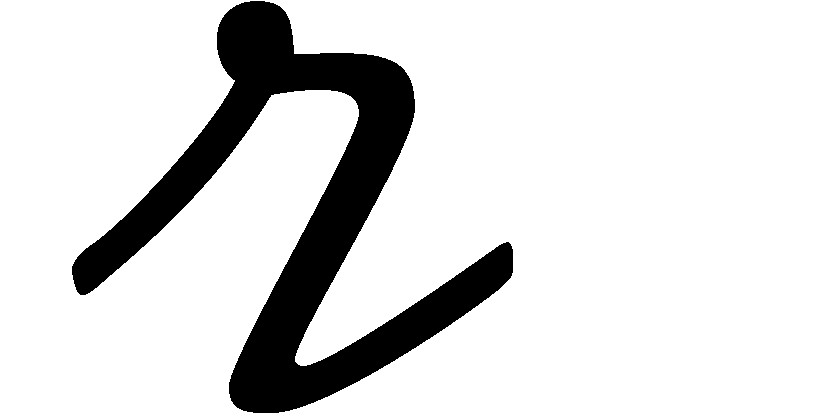
\includegraphics[trim= 1em 0 14em 0,clip]{fonts/ScriptR}}$}}}d^3r'$%
\lthtmlindisplaymathZ
\lthtmlcheckvsize\clearpage}

{\newpage\clearpage
\lthtmlinlinemathA{tex2html_wrap_indisplay3993}%
$\displaystyle \vec{A}(\vec{r}, t)$%
\lthtmlindisplaymathZ
\lthtmlcheckvsize\clearpage}

{\newpage\clearpage
\lthtmlinlinemathA{tex2html_wrap_indisplay3994}%
$\displaystyle = \frac{\mu_0}{4\pi}\int \frac{\vec{J}(\vec{r}', t_r)}{{\mbox{$\resizebox{.09in}{.08in}{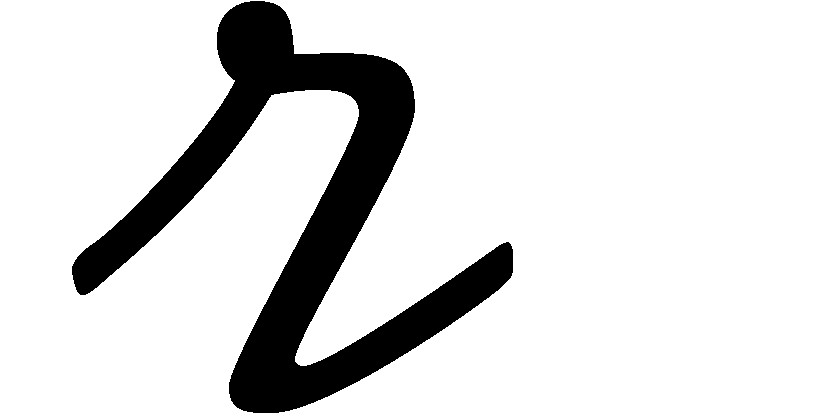
\includegraphics[trim= 1em 0 14em 0,clip]{fonts/ScriptR}}$}}}d^3r'$%
\lthtmlindisplaymathZ
\lthtmlcheckvsize\clearpage}

{\newpage\clearpage
\lthtmlinlinemathA{tex2html_wrap_inline3996}%
$ {\mbox{$\resizebox{.09in}{.08in}{
\includegraphics[trim= 1em 0 14em 0,clip]{fonts/BoldR}}$}}= \vec{r} - \vec{r}'(t_r)$%
\lthtmlindisplaymathZ
\lthtmlcheckvsize\clearpage}

{\newpage\clearpage
\lthtmlinlinemathA{tex2html_wrap_inline3998}%
$ t_r = t -{\mbox{$\resizebox{.09in}{.08in}{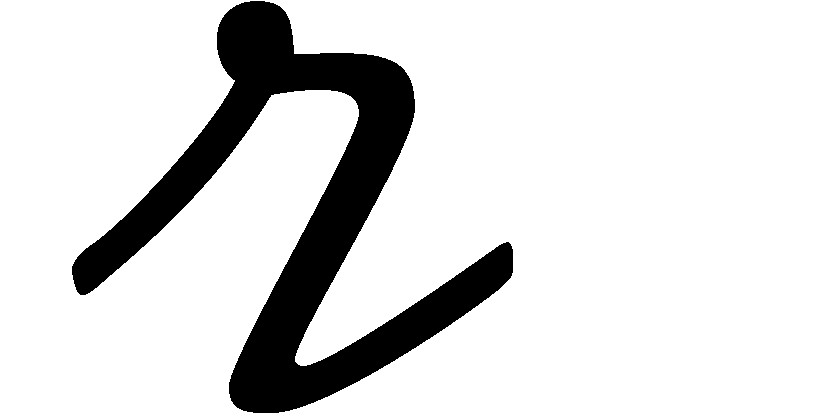
\includegraphics[trim= 1em 0 14em 0,clip]{fonts/ScriptR}}$}}/c$%
\lthtmlindisplaymathZ
\lthtmlcheckvsize\clearpage}

{\newpage\clearpage
\lthtmlinlinemathA{tex2html_wrap_inline4000}%
$ \vec{r}'(t)$%
\lthtmlindisplaymathZ
\lthtmlcheckvsize\clearpage}

{\newpage\clearpage
\lthtmlinlinemathA{tex2html_wrap_indisplay4004}%
$\displaystyle = \frac{1}{4\pi\epsilon_0}    \frac{q}{\left| {\mbox{$\resizebox{.09in}{.08in}{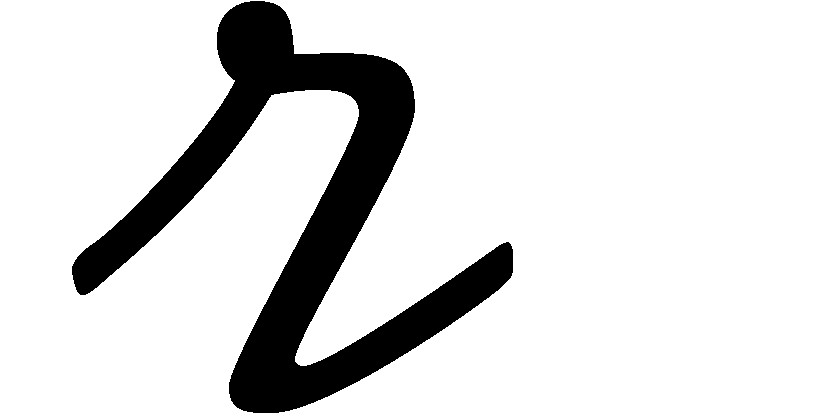
\includegraphics[trim= 1em 0 14em 0,clip]{fonts/ScriptR}}$}}- {\mbox{$\resizebox{.09in}{.08in}{
\includegraphics[trim= 1em 0 14em 0,clip]{fonts/BoldR}}$}}\cdot \vec{\beta} \right|}$%
\lthtmlindisplaymathZ
\lthtmlcheckvsize\clearpage}

{\newpage\clearpage
\lthtmlinlinemathA{tex2html_wrap_indisplay4006}%
$\displaystyle = \frac{\mu_0}{4\pi}    \frac{q\vec{v}}{\left| {\mbox{$\resizebox{.09in}{.08in}{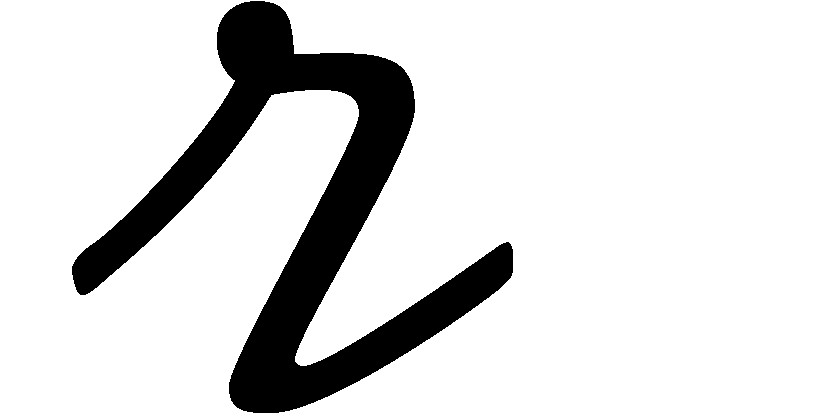
\includegraphics[trim= 1em 0 14em 0,clip]{fonts/ScriptR}}$}}- {\mbox{$\resizebox{.09in}{.08in}{
\includegraphics[trim= 1em 0 14em 0,clip]{fonts/BoldR}}$}}\cdot \vec{\beta} \right|} \;,$%
\lthtmlindisplaymathZ
\lthtmlcheckvsize\clearpage}

{\newpage\clearpage
\lthtmlinlinemathA{tex2html_wrap_inline4008}%
$ \vec{\beta} = \vec{v}/c = \dot{\vec{r}}'(t_r)/c$%
\lthtmlindisplaymathZ
\lthtmlcheckvsize\clearpage}

{\newpage\clearpage
\lthtmlinlinemathA{tex2html_wrap_indisplay4009}%
$\displaystyle \vec{E}(\vec{r}, t)= \frac{q}{4\pi\epsilon_0} \frac{{\mbox{$\resizebox{.09in}{.08in}{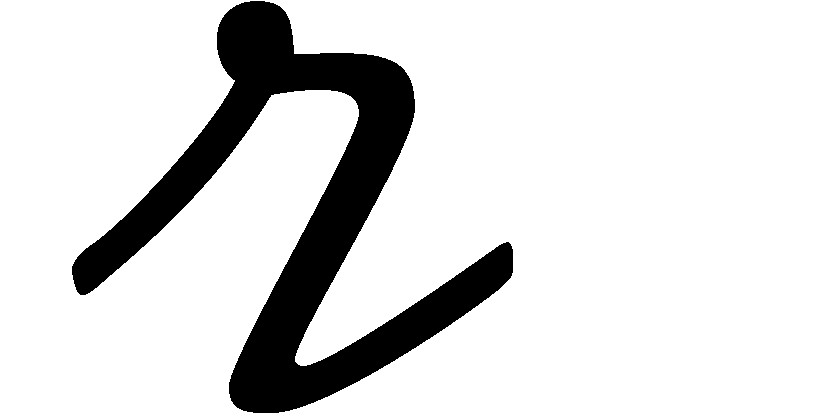
\includegraphics[trim= 1em 0 14em 0,clip]{fonts/ScriptR}}$}}}{({\mbox{$\resizebox{.09in}{.08in}{
\includegraphics[trim= 1em 0 14em 0,clip]{fonts/BoldR}}$}}\cdot \vec{u})^3}
[(c^2 - v^2)\vec{u} + {\mbox{$\resizebox{.09in}{.08in}{
\includegraphics[trim= 1em 0 14em 0,clip]{fonts/BoldR}}$}}\times (\vec{u} \times \vec{a})] \; , \quad\quad \vec{B}(\vec{r}, t)
= \frac{1}{c}{\mbox{$\hat {\mbox{$\resizebox{.09in}{.08in}{
\includegraphics[trim= 1em 0 14em 0,clip]{fonts/BoldR}}$}}$}}\times \vec{E}(\vec{r}, t)$%
\lthtmlindisplaymathZ
\lthtmlcheckvsize\clearpage}

{\newpage\clearpage
\lthtmlinlinemathA{tex2html_wrap_inline4011}%
$ \vec{u} = c {\mbox{$\hat {\mbox{$\resizebox{.09in}{.08in}{
\includegraphics[trim= 1em 0 14em 0,clip]{fonts/BoldR}}$}}$}}- \vec{\beta}$%
\lthtmlindisplaymathZ
\lthtmlcheckvsize\clearpage}

{\newpage\clearpage
\lthtmlinlinemathA{tex2html_wrap_inline4013}%
$ \vec{a}=\ddot{\vec{r}}'(t_r)$%
\lthtmlindisplaymathZ
\lthtmlcheckvsize\clearpage}

\stepcounter{section}
{\newpage\clearpage
\lthtmlinlinemathA{tex2html_wrap_indisplay4015}%
$\displaystyle \vec{E}(\vec r, t) = \vec{E}_$%
\lthtmlindisplaymathZ
\lthtmlcheckvsize\clearpage}

{\newpage\clearpage
\lthtmlinlinemathA{tex2html_wrap_indisplay4016}%
$\displaystyle (\vec r, t) + \vec
E_$%
\lthtmlindisplaymathZ
\lthtmlcheckvsize\clearpage}

{\newpage\clearpage
\lthtmlinlinemathA{tex2html_wrap_indisplay4017}%
$\displaystyle (\vec r, t) \;.$%
\lthtmlindisplaymathZ
\lthtmlcheckvsize\clearpage}

{\newpage\clearpage
\lthtmlinlinemathA{tex2html_wrap_inline4019}%
$ 1/{\mbox{$\resizebox{.09in}{.08in}{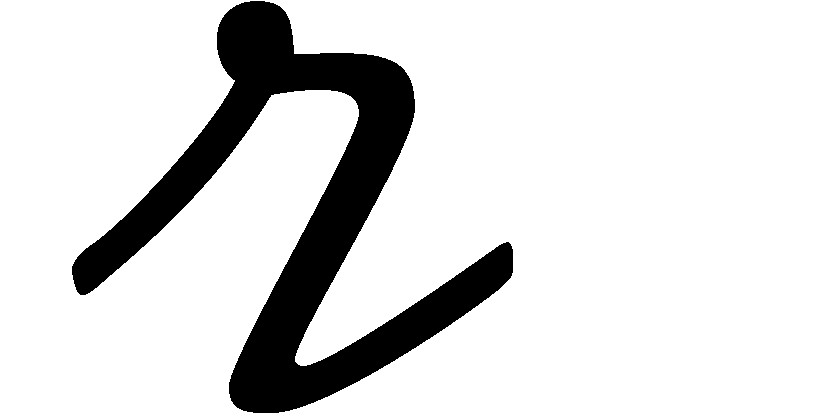
\includegraphics[trim= 1em 0 14em 0,clip]{fonts/ScriptR}}$}}$%
\lthtmlindisplaymathZ
\lthtmlcheckvsize\clearpage}

{\newpage\clearpage
\lthtmlinlinemathA{tex2html_wrap_inline4021}%
$ 1/{\mbox{$\resizebox{.09in}{.08in}{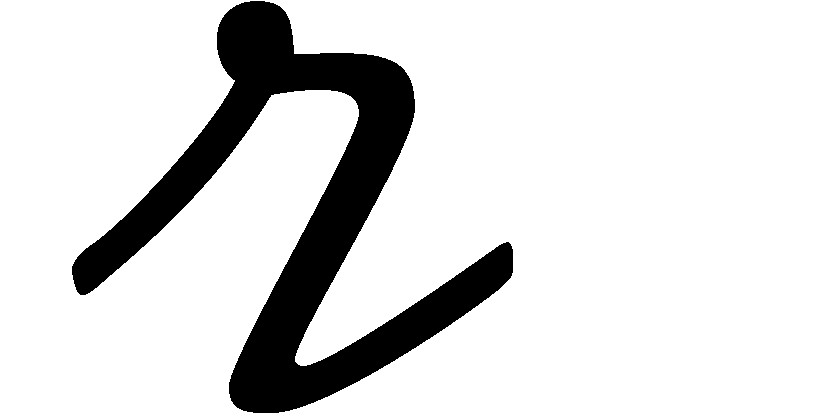
\includegraphics[trim= 1em 0 14em 0,clip]{fonts/ScriptR}}$}}^2$%
\lthtmlindisplaymathZ
\lthtmlcheckvsize\clearpage}

{\newpage\clearpage
\lthtmlinlinemathA{tex2html_wrap_indisplay4022}%
$\displaystyle \vec{E}_$%
\lthtmlindisplaymathZ
\lthtmlcheckvsize\clearpage}

{\newpage\clearpage
\lthtmlinlinemathA{tex2html_wrap_indisplay4023}%
$\displaystyle (\vec r, t) = \frac{q}{4\pi\epsilon_0}
\frac{{\mbox{$\resizebox{.09in}{.08in}{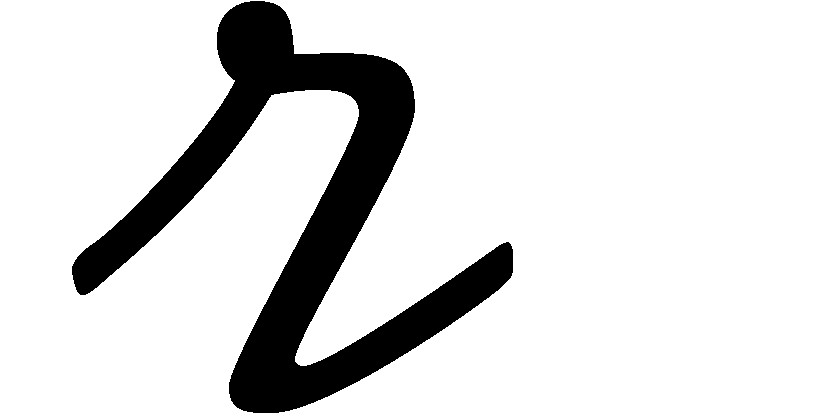
\includegraphics[trim= 1em 0 14em 0,clip]{fonts/ScriptR}}$}}}{({\mbox{$\resizebox{.09in}{.08in}{
\includegraphics[trim= 1em 0 14em 0,clip]{fonts/BoldR}}$}}\cdot \vec{u})^3}
[{\mbox{$\resizebox{.09in}{.08in}{
\includegraphics[trim= 1em 0 14em 0,clip]{fonts/BoldR}}$}}\times (\vec{u} \times \vec{a})] \; , \quad\quad
\vec{B}_\text{rad}(\vec{r}, t)
= \frac{1}{c}{\mbox{$\hat {\mbox{$\resizebox{.09in}{.08in}{
\includegraphics[trim= 1em 0 14em 0,clip]{fonts/BoldR}}$}}$}}\times \vec{E}(\vec{r}, t)$%
\lthtmlindisplaymathZ
\lthtmlcheckvsize\clearpage}

{\newpage\clearpage
\lthtmlinlinemathA{tex2html_wrap_inline4025}%
$ \vec{r}' 
= r_0 \exp(-i\omega t) \hat{\vec{r}}'$%
\lthtmlindisplaymathZ
\lthtmlcheckvsize\clearpage}

{\newpage\clearpage
\lthtmlinlinemathA{tex2html_wrap_inline4027}%
$ r \gg r'$%
\lthtmlindisplaymathZ
\lthtmlcheckvsize\clearpage}

{\newpage\clearpage
\lthtmlinlinemathA{tex2html_wrap_inline4029}%
$ {\mbox{$\resizebox{.09in}{.08in}{
\includegraphics[trim= 1em 0 14em 0,clip]{fonts/BoldR}}$}}\approx \vec{r}$%
\lthtmlindisplaymathZ
\lthtmlcheckvsize\clearpage}

{\newpage\clearpage
\lthtmlinlinemathA{tex2html_wrap_inline4033}%
$ r_0\omega/c = 2\pi r_0/\lambda \ll 1 $%
\lthtmlindisplaymathZ
\lthtmlcheckvsize\clearpage}

{\newpage\clearpage
\lthtmlinlinemathA{tex2html_wrap_inline4035}%
$ v \ll c$%
\lthtmlindisplaymathZ
\lthtmlcheckvsize\clearpage}

{\newpage\clearpage
\lthtmlinlinemathA{tex2html_wrap_inline4037}%
$ \vec{u} \approx c {\mbox{$\hat {\mbox{$\resizebox{.09in}{.08in}{
\includegraphics[trim= 1em 0 14em 0,clip]{fonts/BoldR}}$}}$}}$%
\lthtmlindisplaymathZ
\lthtmlcheckvsize\clearpage}

{\newpage\clearpage
\lthtmlinlinemathA{tex2html_wrap_indisplay4039}%
$\displaystyle (\vec{r},t)$%
\lthtmlindisplaymathZ
\lthtmlcheckvsize\clearpage}

{\newpage\clearpage
\lthtmlinlinemathA{tex2html_wrap_indisplay4040}%
$\displaystyle = \frac{q}{4\pi\epsilon_0} \frac{r}{(\vec{r}\cdot c \hat{\vec{r}})^3}
\vec{r} \times (c \hat{\vec{r}} \times \vec{a})$%
\lthtmlindisplaymathZ
\lthtmlcheckvsize\clearpage}

{\newpage\clearpage
\lthtmlinlinemathA{tex2html_wrap_indisplay4041}%
$\displaystyle = \frac{\mu_0 }{4\pi} \frac{1}{r} \hat{\vec{r}} \times ( \hat{\vec{r}} \times
\ddot{\vec{p}}(t_r))$%
\lthtmlindisplaymathZ
\lthtmlcheckvsize\clearpage}

{\newpage\clearpage
\lthtmlinlinemathA{tex2html_wrap_inline4043}%
$ \vec{p}(t) = q \vec{r}'(t)$%
\lthtmlindisplaymathZ
\lthtmlcheckvsize\clearpage}

{\newpage\clearpage
\lthtmlinlinemathA{tex2html_wrap_indisplay4044}%
$\displaystyle \vec{B}_$%
\lthtmlindisplaymathZ
\lthtmlcheckvsize\clearpage}

{\newpage\clearpage
\lthtmlinlinemathA{tex2html_wrap_indisplay4045}%
$\displaystyle =  \frac{1}{c} \hat{\vec{r}} \times \vec{E}_$%
\lthtmlindisplaymathZ
\lthtmlcheckvsize\clearpage}

{\newpage\clearpage
\lthtmlinlinemathA{tex2html_wrap_indisplay4046}%
$\displaystyle \vec{S} =  \frac{1}{\mu_0} \vec{E}_$%
\lthtmlindisplaymathZ
\lthtmlcheckvsize\clearpage}

{\newpage\clearpage
\lthtmlinlinemathA{tex2html_wrap_indisplay4047}%
$\displaystyle \times\vec{B}_$%
\lthtmlindisplaymathZ
\lthtmlcheckvsize\clearpage}

{\newpage\clearpage
\lthtmlinlinemathA{tex2html_wrap_indisplay4048}%
$\displaystyle =  \frac{1}{\mu_0c} E_$%
\lthtmlindisplaymathZ
\lthtmlcheckvsize\clearpage}

{\newpage\clearpage
\lthtmlinlinemathA{tex2html_wrap_indisplay4049}%
$\displaystyle ^2\hat{\vec{r}}
= \frac{\mu_0}{16 \pi^2 cr^2} |\hat{\vec{r}} \times    \ddot{\vec{p}}|^2\hat{\vec{r}} \;.$%
\lthtmlindisplaymathZ
\lthtmlcheckvsize\clearpage}

{\newpage\clearpage
\lthtmlinlinemathA{tex2html_wrap_inline4051}%
$ d\vec{a} = r^2 \sin\theta d\theta d\phi \hat{\vec{r}} = r^2 d\Omega \hat{\vec{r}}$%
\lthtmlindisplaymathZ
\lthtmlcheckvsize\clearpage}

{\newpage\clearpage
\lthtmlinlinemathA{tex2html_wrap_indisplay4052}%
$\displaystyle dP = \vec{S}\cdot d\vec{a} = \frac{\mu_0 }{16\pi^2 c} |\hat{\vec{r}} \times    \ddot{\vec{p}}|^2 d\Omega \; .$%
\lthtmlindisplaymathZ
\lthtmlcheckvsize\clearpage}

{\newpage\clearpage
\lthtmlinlinemathA{tex2html_wrap_indisplay4053}%
$\displaystyle P = \int \frac{dP}{d\Omega} d\Omega =  \frac{\mu_0 }{16\pi^2 c}  \int |\hat{\vec{r}} \times    \ddot{\vec{p}}|^2 d\Omega  \; .$%
\lthtmlindisplaymathZ
\lthtmlcheckvsize\clearpage}

{\newpage\clearpage
\lthtmlinlinemathA{tex2html_wrap_inline4055}%
$ |\hat{\vec{r}} \times \hat{\vec{p}}|^2 = \sin^2\theta$%
\lthtmlindisplaymathZ
\lthtmlcheckvsize\clearpage}

{\newpage\clearpage
\lthtmlinlinemathA{tex2html_wrap_inline4057}%
$ 8\pi/3$%
\lthtmlindisplaymathZ
\lthtmlcheckvsize\clearpage}

{\newpage\clearpage
\lthtmlinlinemathA{tex2html_wrap_indisplay4058}%
$\displaystyle P =  \frac{\mu_0 \ddot{p}^2}{6\pi c}  \; .$%
\lthtmlindisplaymathZ
\lthtmlcheckvsize\clearpage}

{\newpage\clearpage
\lthtmlinlinemathA{tex2html_wrap_inline4060}%
$ 1/2$%
\lthtmlindisplaymathZ
\lthtmlcheckvsize\clearpage}

{\newpage\clearpage
\lthtmlinlinemathA{tex2html_wrap_indisplay4061}%
$\displaystyle \left\langle dP \right\rangle$%
\lthtmlindisplaymathZ
\lthtmlcheckvsize\clearpage}

{\newpage\clearpage
\lthtmlinlinemathA{tex2html_wrap_indisplay4062}%
$\displaystyle = \frac{\mu_0 \omega^4 p^2}{32\pi^2 c} |\hat{\vec{r}}\times\hat{\vec{p}}|^2 d\Omega$%
\lthtmlindisplaymathZ
\lthtmlcheckvsize\clearpage}

{\newpage\clearpage
\lthtmlinlinemathA{tex2html_wrap_indisplay4063}%
$\displaystyle \langle P \rangle$%
\lthtmlindisplaymathZ
\lthtmlcheckvsize\clearpage}

{\newpage\clearpage
\lthtmlinlinemathA{tex2html_wrap_indisplay4064}%
$\displaystyle =  \frac{\mu_0 \omega^4 p^2}{12\pi c} \; .$%
\lthtmlindisplaymathZ
\lthtmlcheckvsize\clearpage}

\stepcounter{section}
{\newpage\clearpage
\lthtmlinlinemathA{tex2html_wrap_inline4067}%
$ m_e$%
\lthtmlindisplaymathZ
\lthtmlcheckvsize\clearpage}

{\newpage\clearpage
\lthtmlinlinemathA{tex2html_wrap_inline4069}%
$ e$%
\lthtmlindisplaymathZ
\lthtmlcheckvsize\clearpage}

{\newpage\clearpage
\lthtmlinlinemathA{tex2html_wrap_inline4071}%
$ \vec{E}_0(t)$%
\lthtmlindisplaymathZ
\lthtmlcheckvsize\clearpage}

{\newpage\clearpage
\lthtmlinlinemathA{tex2html_wrap_indisplay4072}%
$\displaystyle \vec{a}(t) =  -\frac{e}{m_e} \vec{E}_0(t) \;.$%
\lthtmlindisplaymathZ
\lthtmlcheckvsize\clearpage}

{\newpage\clearpage
\lthtmlinlinemathA{tex2html_wrap_indisplay4073}%
$\displaystyle \ddot{\vec{p}} =  -e \vec{a} = \frac{e^2}{m_e} \vec{E}_0(t) \;.$%
\lthtmlindisplaymathZ
\lthtmlcheckvsize\clearpage}

{\newpage\clearpage
\lthtmlinlinemathA{tex2html_wrap_indisplay4075}%
$\displaystyle =  -\frac{r_e}{r} [\hat{\vec{r}} \times ( \hat{\vec{r}} \times  \vec{E}_0(t_r))]$%
\lthtmlindisplaymathZ
\lthtmlcheckvsize\clearpage}

{\newpage\clearpage
\lthtmlinlinemathA{tex2html_wrap_indisplay4076}%
$\displaystyle r_e = \frac{1}{4\pi \epsilon_0} \frac{e^2}{m_e c^2} \approx 2.8\times10^{-15} \;$%
\lthtmlindisplaymathZ
\lthtmlcheckvsize\clearpage}

{\newpage\clearpage
\lthtmlinlinemathA{tex2html_wrap_indisplay4077}%
$\displaystyle \;.$%
\lthtmlindisplaymathZ
\lthtmlcheckvsize\clearpage}

{\newpage\clearpage
\lthtmlinlinemathA{tex2html_wrap_indisplay4082}%
$\displaystyle \left\langle dP \right\rangle   = \frac{r_e^2 E_0^2}{ 2 \mu_0 c}  |\hat{\vec{r}}\times\hat{\vec{E}}_0|^2 d\Omega
= I_0 r_e^2  |\hat{\vec{r}}\times\hat{\vec{E}}_0|^2  d\Omega   \; .$%
\lthtmlindisplaymathZ
\lthtmlcheckvsize\clearpage}

{\newpage\clearpage
\lthtmlinlinemathA{tex2html_wrap_inline4084}%
$ I_0 = |\hat{\vec{E}}_0|^2/2\mu_0c$%
\lthtmlindisplaymathZ
\lthtmlcheckvsize\clearpage}

{\newpage\clearpage
\lthtmlinlinemathA{tex2html_wrap_indisplay4085}%
$\displaystyle P = \frac{8}{3}\pi r_e^2  I_0  = \sigma_T  I_0$%
\lthtmlindisplaymathZ
\lthtmlcheckvsize\clearpage}

{\newpage\clearpage
\lthtmlinlinemathA{tex2html_wrap_inline4087}%
$ \sigma_T$%
\lthtmlindisplaymathZ
\lthtmlcheckvsize\clearpage}

\stepcounter{section}
{\newpage\clearpage
\lthtmlinlinemathA{tex2html_wrap_inline4090}%
$ \mathcal{P}=| \hat{\vec{r}} 
\times  \hat{\vec{E}}_0 |^2=\sin^2\theta$%
\lthtmlindisplaymathZ
\lthtmlcheckvsize\clearpage}

{\newpage\clearpage
\lthtmlinlinemathA{tex2html_wrap_inline4092}%
$ \hat{\vec{E}}_0$%
\lthtmlindisplaymathZ
\lthtmlcheckvsize\clearpage}

{\newpage\clearpage
\lthtmlinlinemathA{tex2html_wrap_indisplay4093}%
$\displaystyle \vec{E}_0 = \vec{E}_1 + e^{i\phi}\vec{E}_2$%
\lthtmlindisplaymathZ
\lthtmlcheckvsize\clearpage}

{\newpage\clearpage
\lthtmlinlinemathA{tex2html_wrap_inline4095}%
$ \hat{\vec{E}}_2 = \hat{\vec{k}}_0 \times \hat{\vec{E}}_1$%
\lthtmlindisplaymathZ
\lthtmlcheckvsize\clearpage}

{\newpage\clearpage
\lthtmlinlinemathA{tex2html_wrap_indisplay4098}%
$\displaystyle \left\langle \vec{S}(\vec{r}) \right\rangle$%
\lthtmlindisplaymathZ
\lthtmlcheckvsize\clearpage}

{\newpage\clearpage
\lthtmlinlinemathA{tex2html_wrap_indisplay4099}%
$\displaystyle = r_e^2 \frac{1}{r^2} (I_1 | \hat{\vec{r}} \times  \hat{\vec{E}}_1
|^2 + I_2 | \hat{\vec{r}} \times  \hat{\vec{E}}_2 |^2)  \hat{\vec{r}} \;.$%
\lthtmlindisplaymathZ
\lthtmlcheckvsize\clearpage}

{\newpage\clearpage
\lthtmlinlinemathA{tex2html_wrap_indisplay4100}%
$\displaystyle I_0 = I_1 + I_2$%
\lthtmlindisplaymathZ
\lthtmlcheckvsize\clearpage}

{\newpage\clearpage
\lthtmlinlinemathA{tex2html_wrap_inline4102}%
$ \alpha$%
\lthtmlindisplaymathZ
\lthtmlcheckvsize\clearpage}

{\newpage\clearpage
\lthtmlinlinemathA{tex2html_wrap_indisplay4103}%
$\displaystyle I_1$%
\lthtmlindisplaymathZ
\lthtmlcheckvsize\clearpage}

{\newpage\clearpage
\lthtmlinlinemathA{tex2html_wrap_indisplay4104}%
$\displaystyle =\alpha I_0$%
\lthtmlindisplaymathZ
\lthtmlcheckvsize\clearpage}

{\newpage\clearpage
\lthtmlinlinemathA{tex2html_wrap_indisplay4105}%
$\displaystyle I_2$%
\lthtmlindisplaymathZ
\lthtmlcheckvsize\clearpage}

{\newpage\clearpage
\lthtmlinlinemathA{tex2html_wrap_indisplay4106}%
$\displaystyle = (1-\alpha)I_0$%
\lthtmlindisplaymathZ
\lthtmlcheckvsize\clearpage}

{\newpage\clearpage
\lthtmlinlinemathA{tex2html_wrap_indisplay4107}%
$\displaystyle \left\langle dP \right\rangle  = I_0 r_e^2  (\alpha | \hat{\vec{r}} \times  \hat{\vec{E}}_1 |^2 + (1-\alpha)
| \hat{\vec{r}} \times  \hat{\vec{E}}_2 |^2)  d\Omega\;.$%
\lthtmlindisplaymathZ
\lthtmlcheckvsize\clearpage}

{\newpage\clearpage
\lthtmlinlinemathA{tex2html_wrap_indisplay4114}%
$\displaystyle I(\vec{q}) = J_0 r_e^2  \mathcal{P}(\vec{q}) \Delta \Omega$%
\lthtmlindisplaymathZ
\lthtmlcheckvsize\clearpage}

{\newpage\clearpage
\lthtmlinlinemathA{tex2html_wrap_indisplay4115}%
$\displaystyle \mathcal{P}(\vec{q}) = \alpha | \hat{\vec{k}} \times  \hat{\vec{E}}_1 |^2 + (1-\alpha) |
\hat{\vec{k}} \times \hat{\vec{E}}_2 |^2$%
\lthtmlindisplaymathZ
\lthtmlcheckvsize\clearpage}

{\newpage\clearpage
\lthtmlinlinemathA{tex2html_wrap_indisplay4116}%
$\displaystyle \hat{\vec{r}} = \hat{\vec{k}} = \frac{\vec{q} - \vec{k}_0}{\left| \vec{q} - \vec{k}_0 \right|} \;.$%
\lthtmlindisplaymathZ
\lthtmlcheckvsize\clearpage}

{\newpage\clearpage
\lthtmlinlinemathA{tex2html_wrap_indisplay4119}%
$\displaystyle \mathcal{P}(\vec{q})$%
\lthtmlindisplaymathZ
\lthtmlcheckvsize\clearpage}

{\newpage\clearpage
\lthtmlinlinemathA{tex2html_wrap_indisplay4120}%
$\displaystyle = 1 - \alpha(\hat{\vec{k}} \cdot \hat{\vec{E}}_1 )^2 -
(1-\alpha)(\hat{\vec{k}} \cdot \hat{\vec{E}}_2 )^2 \;.$%
\lthtmlindisplaymathZ
\lthtmlcheckvsize\clearpage}

\stepcounter{section}
{\newpage\clearpage
\lthtmlinlinemathA{tex2html_wrap_inline4123}%
$ \vec{r}'$%
\lthtmlindisplaymathZ
\lthtmlcheckvsize\clearpage}

{\newpage\clearpage
\lthtmlinlinemathA{tex2html_wrap_indisplay4124}%
$\displaystyle \vec{E}_0(\vec{r},t) = \vec{E}_0 \exp(i\vec{k}_0 \cdot \vec{r} - i \omega t)$%
\lthtmlindisplaymathZ
\lthtmlcheckvsize\clearpage}

{\newpage\clearpage
\lthtmlinlinemathA{tex2html_wrap_indisplay4126}%
$\displaystyle (\vec{r},t) =  \frac{r_e}{r} [\hat{\vec{r}} \times ( \hat{\vec{r}} \times  \vec{E}_0 )] \exp(i\vec{k}_0 \cdot \vec{r}' - i \omega t_r)$%
\lthtmlindisplaymathZ
\lthtmlcheckvsize\clearpage}

{\newpage\clearpage
\lthtmlinlinemathA{tex2html_wrap_indisplay4131}%
$\displaystyle {\mbox{$\resizebox{.09in}{.08in}{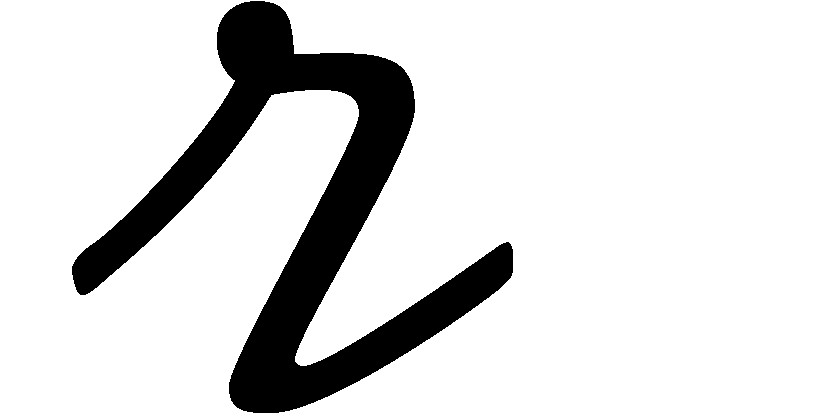
\includegraphics[trim= 1em 0 14em 0,clip]{fonts/ScriptR}}$}}= \sqrt{(\vec{r} - \vec{r}')^2} = \sqrt{r^2 + r'^2 -2\vec{r}\cdot
\vec{r}'} \approx r  - \hat{\vec{r}}\cdot \vec{r}' \;.$%
\lthtmlindisplaymathZ
\lthtmlcheckvsize\clearpage}

{\newpage\clearpage
\lthtmlinlinemathA{tex2html_wrap_inline4133}%
$ t_r \approx t - r/c + \hat{\vec{r}} \cdot \vec r'$%
\lthtmlindisplaymathZ
\lthtmlcheckvsize\clearpage}

{\newpage\clearpage
\lthtmlinlinemathA{tex2html_wrap_indisplay4135}%
$\displaystyle (\vec{r},t) =  \frac{r_e}{r} [\hat{\vec{r}} \times ( \hat{\vec{r}} \times  \vec{E}_0 )]\exp\left(i\vec{k}_0 \cdot \vec{r}' - i\omega t + i \frac{\omega}{c}( r  - \hat{\vec{r}}\cdot \vec{r}')\right) \;.$%
\lthtmlindisplaymathZ
\lthtmlcheckvsize\clearpage}

{\newpage\clearpage
\lthtmlinlinemathA{tex2html_wrap_inline4137}%
$ \vec{k} = \omega/c\; \hat{\vec{r}}=2\pi/\lambda \hat{\vec{r}}$%
\lthtmlindisplaymathZ
\lthtmlcheckvsize\clearpage}

{\newpage\clearpage
\lthtmlinlinemathA{tex2html_wrap_indisplay4141}%
$\displaystyle (\vec{r},t) =  r_e\frac{e^{ikr}}{r} e^{-i\omega t}[\hat{\vec{r}} \times ( \hat{\vec{r}} \times  \vec{E}_0 )]e^{-i\vec{q}\cdot\vec{r}'} \;.$%
\lthtmlindisplaymathZ
\lthtmlcheckvsize\clearpage}

{\newpage\clearpage
\lthtmlinlinemathA{tex2html_wrap_inline4143}%
$ \vec{r}_i'$%
\lthtmlindisplaymathZ
\lthtmlcheckvsize\clearpage}

{\newpage\clearpage
\lthtmlinlinemathA{tex2html_wrap_indisplay4145}%
$\displaystyle (\vec{r},t) =  r_e\frac{e^{ikr}}{r} e^{-i\omega t}[\hat{\vec{r}} \times ( \hat{\vec{r}} \times  \vec{E}_0 )] \sum_i e^{-i\vec{q}\cdot\vec{r}_i'} \;.$%
\lthtmlindisplaymathZ
\lthtmlcheckvsize\clearpage}

{\newpage\clearpage
\lthtmlinlinemathA{tex2html_wrap_indisplay4149}%
$\displaystyle (\vec{r},t) =  r_e\frac{e^{ikr}}{r} e^{-i\omega t}[\hat{\vec{r}} \times ( \hat{\vec{r}} \times  \vec{E}_0 )] \int \rho(\vec{r}') e^{-i\vec{q}\cdot\vec{r}'} d^3r' \;.$%
\lthtmlindisplaymathZ
\lthtmlcheckvsize\clearpage}

{\newpage\clearpage
\lthtmlinlinemathA{tex2html_wrap_indisplay4150}%
$\displaystyle F(\vec{q}) = \int \rho(\vec{r}') e^{-i\vec{q}\cdot\vec{r}'} d^3r' \;.$%
\lthtmlindisplaymathZ
\lthtmlcheckvsize\clearpage}

{\newpage\clearpage
\lthtmlinlinemathA{tex2html_wrap_inline4152}%
$ \vec{q}$%
\lthtmlindisplaymathZ
\lthtmlcheckvsize\clearpage}

{\newpage\clearpage
\lthtmlinlinemathA{tex2html_wrap_indisplay4155}%
$\displaystyle \left\langle \vec{S}(\vec{r}) \right\rangle  = \frac{1}{\mu_0}\left\langle
\Re\{\vec{E}_\text{diff}\}\times\Re\{\vec{B}_\text{diff}\} \right\rangle  = r_e^2
\frac{1}{r^2} J_0 | \hat{\vec{r}} \times  \hat{\vec{E}}_0 |^2 \left| \int \rho(\vec{r}')
e^{-i\vec{q}\cdot\vec{r}'} d^3r' \right|^2 \hat{\vec{r}} \;.$%
\lthtmlindisplaymathZ
\lthtmlcheckvsize\clearpage}

{\newpage\clearpage
\lthtmlinlinemathA{tex2html_wrap_inline4157}%
$ J_0 = |\vec{E}_0|^2/2\mu_0c$%
\lthtmlindisplaymathZ
\lthtmlcheckvsize\clearpage}

{\newpage\clearpage
\lthtmlinlinemathA{tex2html_wrap_inline4159}%
$ d\vec{a} = r^2 d\Omega \hat{\vec{r}}$%
\lthtmlindisplaymathZ
\lthtmlcheckvsize\clearpage}

{\newpage\clearpage
\lthtmlinlinemathA{tex2html_wrap_indisplay4160}%
$\displaystyle I(\vec{q}) = \left\langle \vec{S}(\vec{r}) \right\rangle  \cdot d\vec{a} = r_e^2 J_0 | \hat{\vec{r}} \times
\hat{\vec{E}}_0 |^2 \left| \int \rho(\vec{r}') e^{-i\vec{q}\cdot\vec{r}'} d^3r'
\right|^2 d\Omega\;.$%
\lthtmlindisplaymathZ
\lthtmlcheckvsize\clearpage}

{\newpage\clearpage
\lthtmlinlinemathA{tex2html_wrap_indisplay4161}%
$\displaystyle I(\vec{q}) = J_0 r_e^2  \mathcal{P}(\vec{q})
\left| \int \rho(\vec{r}') e^{-i\vec{q}\cdot\vec{r}'} d^3r' \right|^2 \Delta \Omega \;.$%
\lthtmlindisplaymathZ
\lthtmlcheckvsize\clearpage}

{\newpage\clearpage
\lthtmlinlinemathA{tex2html_wrap_inline4163}%
$ F(\vec{q})$%
\lthtmlindisplaymathZ
\lthtmlcheckvsize\clearpage}

\stepcounter{section}
{\newpage\clearpage
\lthtmlinlinemathA{tex2html_wrap_inline4166}%
$ \vec{x}$%
\lthtmlindisplaymathZ
\lthtmlcheckvsize\clearpage}

{\newpage\clearpage
\lthtmlinlinemathA{tex2html_wrap_indisplay4167}%
$\displaystyle m_e \frac{d^2\vec{x}}{dt^2} + m_e \gamma \frac{d\vec{x}}{dt} + m_e\omega_0^2
\vec{x} = e \vec{E}_0 \exp(-i\omega t) \;.$%
\lthtmlindisplaymathZ
\lthtmlcheckvsize\clearpage}

{\newpage\clearpage
\lthtmlinlinemathA{tex2html_wrap_inline4169}%
$ \vec{x}(t)$%
\lthtmlindisplaymathZ
\lthtmlcheckvsize\clearpage}

{\newpage\clearpage
\lthtmlinlinemathA{tex2html_wrap_indisplay4170}%
$\displaystyle \vec{p}(t) = e \vec{x}(t) = \frac{e^2/m_e}{\omega_0^2 - \omega^2 - i \gamma
\omega}\vec{E}_0 \exp(-i\omega t) \;.$%
\lthtmlindisplaymathZ
\lthtmlcheckvsize\clearpage}

{\newpage\clearpage
\lthtmlinlinemathA{tex2html_wrap_indisplay4172}%
$\displaystyle =  -\frac{\omega^2}{\omega_0^2 - \omega^2 - i \gamma
\omega}\frac{r_e}{r} [\hat{\vec{r}} \times ( \hat{\vec{r}} \times
\vec{E}_0(t_r))] \;$%
\lthtmlindisplaymathZ
\lthtmlcheckvsize\clearpage}

{\newpage\clearpage
\lthtmlinlinemathA{tex2html_wrap_inline4174}%
$ \omega$%
\lthtmlindisplaymathZ
\lthtmlcheckvsize\clearpage}

\stepcounter{section}
{\newpage\clearpage
\lthtmlinlinemathA{tex2html_wrap_inline4177}%
$ \rho_n^{(0)}(r)$%
\lthtmlindisplaymathZ
\lthtmlcheckvsize\clearpage}

{\newpage\clearpage
\lthtmlinlinemathA{tex2html_wrap_indisplay4182}%
$\displaystyle f_n^{(0)}(q)  = \int_{-\infty}^\infty \rho_n^{(0)}(r) \exp(-i
\vec{q}\cdot\vec{r}) \; d^3r = \int_0^\infty \rho_n^{(0)}(r)
\frac{\sin(qr)}{qr}  4\pi r^2 dr \; .$%
\lthtmlindisplaymathZ
\lthtmlcheckvsize\clearpage}

{\newpage\clearpage
\lthtmlinlinemathA{tex2html_wrap_inline4184}%
$ \vec{r}_n$%
\lthtmlindisplaymathZ
\lthtmlcheckvsize\clearpage}

{\newpage\clearpage
\lthtmlinlinemathA{tex2html_wrap_indisplay4185}%
$\displaystyle f_n^{(0)}(\vec{q})  = \int_{-\infty}^\infty \rho_n(|\vec{r}-\vec{r}_n|) \exp(-i
\vec{q}\cdot\vec{r}) d^3r = f_n^{(0)}(q)
\exp(-i \vec{q}\cdot\vec{r}_n)  \; .$%
\lthtmlindisplaymathZ
\lthtmlcheckvsize\clearpage}

{\newpage\clearpage
\lthtmlinlinemathA{tex2html_wrap_indisplay4186}%
$\displaystyle f_n(q) = f_n^{(0)}(q) + \Delta f_n(E) = f_n^{(0)}(q) + f_n'(E) + i f_n''(E)  \;.$%
\lthtmlindisplaymathZ
\lthtmlcheckvsize\clearpage}

{\newpage\clearpage
\lthtmlinlinemathA{tex2html_wrap_indisplay4187}%
$\displaystyle F(\vec{q})  = \sum_n f_n(q)
e^{-i \vec{q}\cdot\vec{r}_n}  \; .$%
\lthtmlindisplaymathZ
\lthtmlcheckvsize\clearpage}

{\newpage\clearpage
\lthtmlinlinemathA{tex2html_wrap_indisplay4188}%
$\displaystyle \rho(\vec{r})$%
\lthtmlindisplaymathZ
\lthtmlcheckvsize\clearpage}

{\newpage\clearpage
\lthtmlinlinemathA{tex2html_wrap_indisplay4189}%
$\displaystyle = \sum_n^N \rho_n^{(0)}(|\vec{r}-\vec{r}_n|) +
\delta(\vec{r}-\vec{r}_n) \Delta f_n(E) \; .$%
\lthtmlindisplaymathZ
\lthtmlcheckvsize\clearpage}

\stepcounter{section}
{\newpage\clearpage
\lthtmlinlinemathA{tex2html_wrap_inline4192}%
$ N$%
\lthtmlindisplaymathZ
\lthtmlcheckvsize\clearpage}

{\newpage\clearpage
\lthtmlinlinemathA{tex2html_wrap_indisplay4193}%
$\displaystyle \vec{P}(t) = N \frac{e^2/m_e}{\omega_0^2 - \omega^2 - i \gamma \omega}\vec{E}_0
\exp(-i\omega t) \;.$%
\lthtmlindisplaymathZ
\lthtmlcheckvsize\clearpage}

{\newpage\clearpage
\lthtmlinlinemathA{tex2html_wrap_inline4195}%
$ \vec{P} = \epsilon_0 \chi_e 
\vec{E}$%
\lthtmlindisplaymathZ
\lthtmlcheckvsize\clearpage}

{\newpage\clearpage
\lthtmlinlinemathA{tex2html_wrap_inline4197}%
$ \epsilon = \epsilon_0 (1+\chi_e)$%
\lthtmlindisplaymathZ
\lthtmlcheckvsize\clearpage}

{\newpage\clearpage
\lthtmlinlinemathA{tex2html_wrap_inline4199}%
$ n = 
\sqrt{\epsilon/\epsilon_0}$%
\lthtmlindisplaymathZ
\lthtmlcheckvsize\clearpage}

{\newpage\clearpage
\lthtmlinlinemathA{tex2html_wrap_indisplay4200}%
$\displaystyle n = \sqrt{1+N \frac{e^2/m_e\epsilon_0}{\omega_0^2 - \omega^2 - i
\gamma \omega}}$%
\lthtmlindisplaymathZ
\lthtmlcheckvsize\clearpage}

{\newpage\clearpage
\lthtmlinlinemathA{tex2html_wrap_indisplay4201}%
$\displaystyle n \approx 1 - \frac{N e^2}{2 m \epsilon_0 \omega^2}  \;.$%
\lthtmlindisplaymathZ
\lthtmlcheckvsize\clearpage}

{\newpage\clearpage
\lthtmlinlinemathA{tex2html_wrap_inline4203}%
$ r_e$%
\lthtmlindisplaymathZ
\lthtmlcheckvsize\clearpage}

{\newpage\clearpage
\lthtmlinlinemathA{tex2html_wrap_indisplay4204}%
$\displaystyle n \approx 1 - \frac{1}{2\pi} r_e N \lambda^2 \;.$%
\lthtmlindisplaymathZ
\lthtmlcheckvsize\clearpage}

{\newpage\clearpage
\lthtmlinlinemathA{tex2html_wrap_indisplay4205}%
$\displaystyle n(\vec{r}) \approx 1 - \frac{1}{2\pi} r_e \rho(\vec{r}) \lambda^2 \;.$%
\lthtmlindisplaymathZ
\lthtmlcheckvsize\clearpage}

\appendix
\stepcounter{section}
{\newpage\clearpage
\lthtmlinlinemathA{tex2html_wrap_inline4208}%
$ V(\vec{r}, t)$%
\lthtmlindisplaymathZ
\lthtmlcheckvsize\clearpage}

{\newpage\clearpage
\lthtmlinlinemathA{tex2html_wrap_indisplay4209}%
$\displaystyle \nabla^2 V(\vec{r}, t) - \mu_0\epsilon_0 \frac{\partial^2 V(\vec{r}, t)}{\partial t^2}$%
\lthtmlindisplaymathZ
\lthtmlcheckvsize\clearpage}

{\newpage\clearpage
\lthtmlinlinemathA{tex2html_wrap_indisplay4210}%
$\displaystyle = -\rho(\vec{r}, t) / \epsilon_0$%
\lthtmlindisplaymathZ
\lthtmlcheckvsize\clearpage}

{\newpage\clearpage
\lthtmlinlinemathA{tex2html_wrap_inline4212}%
$ \rho(\vec{r}, t)$%
\lthtmlindisplaymathZ
\lthtmlcheckvsize\clearpage}

{\newpage\clearpage
\lthtmlinlinemathA{tex2html_wrap_inline4214}%
$ \vec{A}$%
\lthtmlindisplaymathZ
\lthtmlcheckvsize\clearpage}

{\newpage\clearpage
\lthtmlinlinemathA{tex2html_wrap_inline4216}%
$ \mathcal{L}_{\vec{r}}$%
\lthtmlindisplaymathZ
\lthtmlcheckvsize\clearpage}

{\newpage\clearpage
\lthtmlinlinemathA{tex2html_wrap_inline4218}%
$ V(\vec{r})$%
\lthtmlindisplaymathZ
\lthtmlcheckvsize\clearpage}

{\newpage\clearpage
\lthtmlinlinemathA{tex2html_wrap_indisplay4219}%
$\displaystyle \mathcal{L}_{\vec{r}} V(\vec{r}) = g(\vec{r}) \;.$%
\lthtmlindisplaymathZ
\lthtmlcheckvsize\clearpage}

{\newpage\clearpage
\lthtmlinlinemathA{tex2html_wrap_inline4221}%
$ \vec r$%
\lthtmlindisplaymathZ
\lthtmlcheckvsize\clearpage}

{\newpage\clearpage
\lthtmlinlinemathA{tex2html_wrap_inline4223}%
$ G(\vec{r}, \vec{r}')$%
\lthtmlindisplaymathZ
\lthtmlcheckvsize\clearpage}

{\newpage\clearpage
\lthtmlinlinemathA{tex2html_wrap_indisplay4224}%
$\displaystyle \mathcal{L}_{\vec{r}} G(\vec{r}, \vec{r}') = \delta(\vec{r}-\vec{r}')$%
\lthtmlindisplaymathZ
\lthtmlcheckvsize\clearpage}

{\newpage\clearpage
\lthtmlinlinemathA{tex2html_wrap_inline4226}%
$ \delta(\vec{r}-\vec{r}')$%
\lthtmlindisplaymathZ
\lthtmlcheckvsize\clearpage}

{\newpage\clearpage
\lthtmlinlinemathA{tex2html_wrap_indisplay4231}%
$\displaystyle V(\vec{r}) = \int_{\text{Vol}} g(\vec{r}')G(\vec{r}, \vec{r}') d^3 r'\;.$%
\lthtmlindisplaymathZ
\lthtmlcheckvsize\clearpage}

{\newpage\clearpage
\lthtmlinlinemathA{tex2html_wrap_indisplay4234}%
$\displaystyle \mathcal{L}_{\vec{r}} V(\vec{r})$%
\lthtmlindisplaymathZ
\lthtmlcheckvsize\clearpage}

{\newpage\clearpage
\lthtmlinlinemathA{tex2html_wrap_indisplay4235}%
$\displaystyle = \mathcal{L}_{\vec{r}} \int_{\text{Vol}} g(\vec{r}')G(\vec{r}, \vec{r}')d^3 r'$%
\lthtmlindisplaymathZ
\lthtmlcheckvsize\clearpage}

{\newpage\clearpage
\lthtmlinlinemathA{tex2html_wrap_indisplay4236}%
$\displaystyle = \int_{\text{Vol}} g(\vec{r}')  \mathcal{L}_{\vec{r}} G(\vec{r}, \vec{r}') d^3 r'$%
\lthtmlindisplaymathZ
\lthtmlcheckvsize\clearpage}

{\newpage\clearpage
\lthtmlinlinemathA{tex2html_wrap_indisplay4237}%
$\displaystyle = \int_{\text{Vol}} g(\vec{r}')  \delta(\vec{r} - \vec{r}') d^3 r'$%
\lthtmlindisplaymathZ
\lthtmlcheckvsize\clearpage}

{\newpage\clearpage
\lthtmlinlinemathA{tex2html_wrap_indisplay4239}%
$\displaystyle = g(\vec{r})$%
\lthtmlindisplaymathZ
\lthtmlcheckvsize\clearpage}

{\newpage\clearpage
\lthtmlinlinemathA{tex2html_wrap_indisplay4245}%
$\displaystyle = \int_{-\infty}^{\infty} V_{\omega}(\vec{r})e^{- i\omega t} d\omega$%
\lthtmlindisplaymathZ
\lthtmlcheckvsize\clearpage}

{\newpage\clearpage
\lthtmlinlinemathA{tex2html_wrap_indisplay4246}%
$\displaystyle \rho(\vec{r}, t)$%
\lthtmlindisplaymathZ
\lthtmlcheckvsize\clearpage}

{\newpage\clearpage
\lthtmlinlinemathA{tex2html_wrap_indisplay4247}%
$\displaystyle = \int_{-\infty}^{\infty} \rho_{\omega}(\vec{r})e^{- i\omega t} d\omega \;.$%
\lthtmlindisplaymathZ
\lthtmlcheckvsize\clearpage}

{\newpage\clearpage
\lthtmlinlinemathA{tex2html_wrap_indisplay4248}%
$\displaystyle (\nabla^2 + k^2) V_\omega(\vec{r}) = -\rho_\omega (\vec{r})/\epsilon_0$%
\lthtmlindisplaymathZ
\lthtmlcheckvsize\clearpage}

{\newpage\clearpage
\lthtmlinlinemathA{tex2html_wrap_inline4250}%
$ k = \sqrt{\mu_0\epsilon_0}\omega$%
\lthtmlindisplaymathZ
\lthtmlcheckvsize\clearpage}

{\newpage\clearpage
\lthtmlinlinemathA{tex2html_wrap_indisplay4251}%
$\displaystyle (\nabla^2 + k^2)G(\vec{r}, \vec{r}') = \delta(\vec{r}-\vec{r}')$%
\lthtmlindisplaymathZ
\lthtmlcheckvsize\clearpage}

{\newpage\clearpage
\lthtmlinlinemathA{tex2html_wrap_inline4253}%
$ \vec{R} = \vec{r}-\vec{r}'$%
\lthtmlindisplaymathZ
\lthtmlcheckvsize\clearpage}

{\newpage\clearpage
\lthtmlinlinemathA{tex2html_wrap_indisplay4254}%
$\displaystyle (\nabla^2 + k^2)G(\vec{r}, \vec{r}') = \delta(\vec{R})$%
\lthtmlindisplaymathZ
\lthtmlcheckvsize\clearpage}

{\newpage\clearpage
\lthtmlinlinemathA{tex2html_wrap_inline4256}%
$ \vec{R}$%
\lthtmlindisplaymathZ
\lthtmlcheckvsize\clearpage}

{\newpage\clearpage
\lthtmlinlinemathA{tex2html_wrap_inline4258}%
$ G(\vec{r}, \vec{r}') = G(R)$%
\lthtmlindisplaymathZ
\lthtmlcheckvsize\clearpage}

{\newpage\clearpage
\lthtmlinlinemathA{tex2html_wrap_indisplay4259}%
$\displaystyle \left(\frac{1}{R}\frac{\partial}{\partial R}R + k^2\right)G(R) = \delta(R) \;.$%
\lthtmlindisplaymathZ
\lthtmlcheckvsize\clearpage}

{\newpage\clearpage
\lthtmlinlinemathA{tex2html_wrap_inline4261}%
$ R \ne 0$%
\lthtmlindisplaymathZ
\lthtmlcheckvsize\clearpage}

{\newpage\clearpage
\lthtmlinlinemathA{tex2html_wrap_inline4263}%
$ \delta(R)=0$%
\lthtmlindisplaymathZ
\lthtmlcheckvsize\clearpage}

{\newpage\clearpage
\lthtmlinlinemathA{tex2html_wrap_indisplay4264}%
$\displaystyle \frac{\partial}{\partial R}[RG(R)] =- k^2 [R G(R)]$%
\lthtmlindisplaymathZ
\lthtmlcheckvsize\clearpage}

{\newpage\clearpage
\lthtmlinlinemathA{tex2html_wrap_indisplay4265}%
$\displaystyle G(R) = A \frac{e^{ikR}}{R} + B \frac{e^{-ikR}}{R} \;.$%
\lthtmlindisplaymathZ
\lthtmlcheckvsize\clearpage}

{\newpage\clearpage
\lthtmlinlinemathA{tex2html_wrap_inline4267}%
$ B=0$%
\lthtmlindisplaymathZ
\lthtmlcheckvsize\clearpage}

{\newpage\clearpage
\lthtmlinlinemathA{tex2html_wrap_inline4269}%
$ A$%
\lthtmlindisplaymathZ
\lthtmlcheckvsize\clearpage}

{\newpage\clearpage
\lthtmlinlinemathA{tex2html_wrap_indisplay4270}%
$\displaystyle \int_{\text{sphere}}\nabla^2 G(R) d^3R  + k^2 \int_\text{sphere} G(R) d^3R = 1 \;.$%
\lthtmlindisplaymathZ
\lthtmlcheckvsize\clearpage}

{\newpage\clearpage
\lthtmlinlinemathA{tex2html_wrap_inline4272}%
$ R\rightarrow 0$%
\lthtmlindisplaymathZ
\lthtmlcheckvsize\clearpage}

{\newpage\clearpage
\lthtmlinlinemathA{tex2html_wrap_inline4274}%
$ G(R) \rightarrow A/R$%
\lthtmlindisplaymathZ
\lthtmlcheckvsize\clearpage}

{\newpage\clearpage
\lthtmlinlinemathA{tex2html_wrap_indisplay4275}%
$\displaystyle A \int_{\text{sphere}}\nabla^2 \frac{1}{R} d^3R  + A k^2 \int_\text{sphere} \frac{1}{R} 4\pi R^2dR = 1 \;.$%
\lthtmlindisplaymathZ
\lthtmlcheckvsize\clearpage}

{\newpage\clearpage
\lthtmlinlinemathA{tex2html_wrap_inline4277}%
$ \nabla^2 (1/R) = -4\pi \delta(R)$%
\lthtmlindisplaymathZ
\lthtmlcheckvsize\clearpage}

{\newpage\clearpage
\lthtmlinlinemathA{tex2html_wrap_indisplay4278}%
$\displaystyle A = -\frac{1}{4\pi} \;.$%
\lthtmlindisplaymathZ
\lthtmlcheckvsize\clearpage}

{\newpage\clearpage
\lthtmlinlinemathA{tex2html_wrap_indisplay4279}%
$\displaystyle G(\vec{r}, \vec{r}') = - \frac{e^{ik|\vec{r}-\vec{r}'|}}{4\pi
|\vec{r}-\vec{r}'|} \;.$%
\lthtmlindisplaymathZ
\lthtmlcheckvsize\clearpage}

{\newpage\clearpage
\lthtmlinlinemathA{tex2html_wrap_indisplay4280}%
$\displaystyle V_\omega(\vec{r}) = \int_{\text{Vol}} \frac{\rho_\omega(\vec{r}')}{4\pi \epsilon_0} \frac{e^{ik|\vec{r}-\vec{r}'|}}{ |\vec{r}-\vec{r}'|} d^3 r'\;.$%
\lthtmlindisplaymathZ
\lthtmlcheckvsize\clearpage}

{\newpage\clearpage
\lthtmlinlinemathA{tex2html_wrap_indisplay4282}%
$\displaystyle = \int_{-\infty}^\infty \left\{\int_{\text{Vol}} \frac{\rho_\omega(\vec{r}')}{4\pi \epsilon_0} \frac{e^{ik|\vec{r}-\vec{r}'|}}{ |\vec{r}-\vec{r}'|} d^3 r' \right\}e^{-i\omega t}d\omega$%
\lthtmlindisplaymathZ
\lthtmlcheckvsize\clearpage}

{\newpage\clearpage
\lthtmlinlinemathA{tex2html_wrap_indisplay4283}%
$\displaystyle =\int_{\text{Vol}} \left\{ \int_{-\infty}^\infty\rho_\omega(\vec{r}') e^{-i\omega (t -|\vec{r}-\vec{r}'|/c)} d\omega\right\}\frac{1}{4\pi \epsilon_0} \frac{1}{ |\vec{r}-\vec{r}'|} d^3 r'  \;.$%
\lthtmlindisplaymathZ
\lthtmlcheckvsize\clearpage}

{\newpage\clearpage
\lthtmlinlinemathA{tex2html_wrap_indisplay4286}%
$\displaystyle t_r \equiv t - {\mbox{$\resizebox{.09in}{.08in}{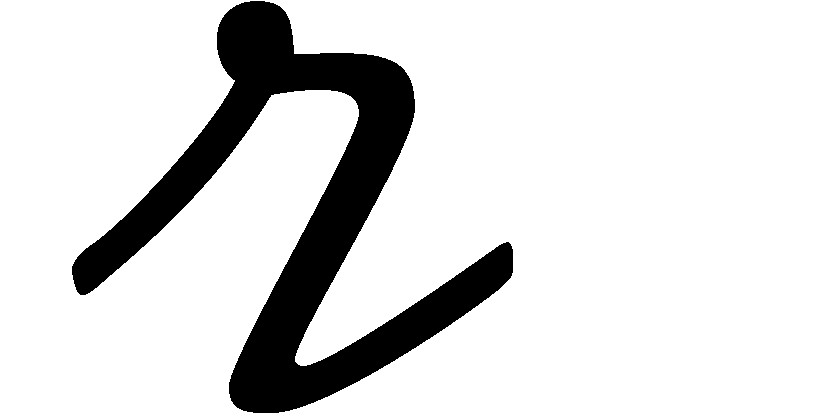
\includegraphics[trim= 1em 0 14em 0,clip]{fonts/ScriptR}}$}}/ c \;.$%
\lthtmlindisplaymathZ
\lthtmlcheckvsize\clearpage}

\stepcounter{section}
{\newpage\clearpage
\lthtmlinlinemathA{tex2html_wrap_inline4289}%
$ \vec{w}(t)$%
\lthtmlindisplaymathZ
\lthtmlcheckvsize\clearpage}

{\newpage\clearpage
\lthtmlinlinemathA{tex2html_wrap_inline4291}%
$ \vec{r}$%
\lthtmlindisplaymathZ
\lthtmlcheckvsize\clearpage}

{\newpage\clearpage
\lthtmlinlinemathA{tex2html_wrap_indisplay4292}%
$\displaystyle V(\vec{r}, t) = \frac{1}{4\pi\epsilon_0}\int \frac{\rho(\vec{r}', t_r)}{|\vec{r} - \vec{r}'|} d^3r'$%
\lthtmlindisplaymathZ
\lthtmlcheckvsize\clearpage}

{\newpage\clearpage
\lthtmlinlinemathA{tex2html_wrap_indisplay4293}%
$\displaystyle t_r(t, \vec{r}') \equiv t - |\vec{r}-\vec{r}'|/c$%
\lthtmlindisplaymathZ
\lthtmlcheckvsize\clearpage}

{\newpage\clearpage
\lthtmlinlinemathA{tex2html_wrap_indisplay4295}%
$\displaystyle = q \delta(\vec{r} - \vec{w}(t))$%
\lthtmlindisplaymathZ
\lthtmlcheckvsize\clearpage}

{\newpage\clearpage
\lthtmlinlinemathA{tex2html_wrap_indisplay4296}%
$\displaystyle = q \int  \delta(\vec{r} - \vec{w}(t')) \delta(t' - t_r(t, \vec{r}'))  dt'$%
\lthtmlindisplaymathZ
\lthtmlcheckvsize\clearpage}

{\newpage\clearpage
\lthtmlinlinemathA{tex2html_wrap_indisplay4297}%
$\displaystyle V(\vec{r}, t) = \frac{q}{4\pi\epsilon_0}\iint \frac{  \delta(\vec{r}' - \vec{w}(t')) \delta(t' - t_r(t, \vec{r}'))  }{|\vec{r} - \vec{r}'|} d^3r' dt'$%
\lthtmlindisplaymathZ
\lthtmlcheckvsize\clearpage}

{\newpage\clearpage
\lthtmlinlinemathA{tex2html_wrap_inline4299}%
$ t$%
\lthtmlindisplaymathZ
\lthtmlcheckvsize\clearpage}

{\newpage\clearpage
\lthtmlinlinemathA{tex2html_wrap_inline4301}%
$ t'$%
\lthtmlindisplaymathZ
\lthtmlcheckvsize\clearpage}

{\newpage\clearpage
\lthtmlinlinemathA{tex2html_wrap_inline4309}%
$ t_r(t, \vec{r}')$%
\lthtmlindisplaymathZ
\lthtmlcheckvsize\clearpage}

{\newpage\clearpage
\lthtmlinlinemathA{tex2html_wrap_indisplay4310}%
$\displaystyle V(\vec{r}, t) = \frac{q}{4\pi\epsilon_0}\int \frac{ \delta(t' - t_r(t, \vec{w}(t') )\;)  }{|\vec{r} - \vec{w}(t')|} dt'$%
\lthtmlindisplaymathZ
\lthtmlcheckvsize\clearpage}

{\newpage\clearpage
\lthtmlinlinemathA{tex2html_wrap_indisplay4311}%
$\displaystyle \delta(g(x))$%
\lthtmlindisplaymathZ
\lthtmlcheckvsize\clearpage}

{\newpage\clearpage
\lthtmlinlinemathA{tex2html_wrap_indisplay4312}%
$\displaystyle = \frac{\delta(x-x')}{|g'(x')|}$%
\lthtmlindisplaymathZ
\lthtmlcheckvsize\clearpage}

{\newpage\clearpage
\lthtmlinlinemathA{tex2html_wrap_inline4314}%
$ x'$%
\lthtmlindisplaymathZ
\lthtmlcheckvsize\clearpage}

{\newpage\clearpage
\lthtmlinlinemathA{tex2html_wrap_indisplay4315}%
$\displaystyle g(x')$%
\lthtmlindisplaymathZ
\lthtmlcheckvsize\clearpage}

{\newpage\clearpage
\lthtmlinlinemathA{tex2html_wrap_inline4318}%
$ g'(x)$%
\lthtmlindisplaymathZ
\lthtmlcheckvsize\clearpage}

{\newpage\clearpage
\lthtmlinlinemathA{tex2html_wrap_indisplay4319}%
$\displaystyle g'(x)$%
\lthtmlindisplaymathZ
\lthtmlcheckvsize\clearpage}

{\newpage\clearpage
\lthtmlinlinemathA{tex2html_wrap_indisplay4320}%
$\displaystyle \equiv \frac{d }{dx}g(x)  \;.$%
\lthtmlindisplaymathZ
\lthtmlcheckvsize\clearpage}

{\newpage\clearpage
\lthtmlinlinemathA{tex2html_wrap_indisplay4321}%
$\displaystyle \delta(t' - t_r(t, \vec{w}(t') )\;) = \frac{\delta(t' - t^*)}{\left |  \frac{d}{dt'} \left(  t' - \left(t - \frac{|\vec{r} - \vec{w}(t')|}{c}\right) \right)_{t' = t^*} \right |}$%
\lthtmlindisplaymathZ
\lthtmlcheckvsize\clearpage}

{\newpage\clearpage
\lthtmlinlinemathA{tex2html_wrap_indisplay4322}%
$\displaystyle \frac{d}{dt'} \left(  t' - \left(t - \frac{|\vec{r} - \vec{w}(t')|}{c}\right) \right)$%
\lthtmlindisplaymathZ
\lthtmlcheckvsize\clearpage}

{\newpage\clearpage
\lthtmlinlinemathA{tex2html_wrap_indisplay4323}%
$\displaystyle = 1 + \frac{1}{c} \frac{d}{dt'} |\vec{r} - \vec{w}(t')|$%
\lthtmlindisplaymathZ
\lthtmlcheckvsize\clearpage}

{\newpage\clearpage
\lthtmlinlinemathA{tex2html_wrap_indisplay4324}%
$\displaystyle = 1 + \frac{1}{c} \frac{d}{dt'} \left( \left( \vec{r} - \vec{w}(t')\right)^2 \right)^{1/2}$%
\lthtmlindisplaymathZ
\lthtmlcheckvsize\clearpage}

{\newpage\clearpage
\lthtmlinlinemathA{tex2html_wrap_indisplay4325}%
$\displaystyle = 1 + \frac{1}{2c} \frac{1}{ |\vec{r} - \vec{w}(t')| } \frac{d}{dt'}\left( \vec{r} - \vec{w}(t')\right)^2$%
\lthtmlindisplaymathZ
\lthtmlcheckvsize\clearpage}

{\newpage\clearpage
\lthtmlinlinemathA{tex2html_wrap_indisplay4326}%
$\displaystyle = 1 + \frac{1}{2c} \frac{1}{ |\vec{r} - \vec{w}(t')| } \frac{d}{dt'}\left( \vec{r}\cdot \vec{r} + \vec{w}(t')\cdot \vec{w}(t') - 2\vec{r} \cdot \vec{w}(t')\right)$%
\lthtmlindisplaymathZ
\lthtmlcheckvsize\clearpage}

{\newpage\clearpage
\lthtmlinlinemathA{tex2html_wrap_indisplay4327}%
$\displaystyle = 1 + \frac{1}{2c} \frac{1}{ |\vec{r} - \vec{w}(t')| } \left( 2 \vec{w}(t')\cdot  \dot{\vec{w}}(t') - 2\vec{r} \cdot
\dot{\vec{w}}(t')\right)$%
\lthtmlindisplaymathZ
\lthtmlcheckvsize\clearpage}

{\newpage\clearpage
\lthtmlinlinemathA{tex2html_wrap_indisplay4328}%
$\displaystyle = 1 - \frac{1}{c} \frac{ \left( \vec{r} \cdot
\dot{\vec{w}}(t') - \vec{w}(t')\cdot  \dot{\vec{w}}(t') \right)  }{ |\vec{r} - \vec{w}(t')| }$%
\lthtmlindisplaymathZ
\lthtmlcheckvsize\clearpage}

{\newpage\clearpage
\lthtmlinlinemathA{tex2html_wrap_indisplay4329}%
$\displaystyle = 1 - \frac{1}{c} \frac{ \left( \vec{r}  - \vec{w}(t')  \right)\cdot  \dot{\vec{w}}(t') }{ |\vec{r} - \vec{w}(t')| }$%
\lthtmlindisplaymathZ
\lthtmlcheckvsize\clearpage}

{\newpage\clearpage
\lthtmlinlinemathA{tex2html_wrap_inline4331}%
$ t^*$%
\lthtmlindisplaymathZ
\lthtmlcheckvsize\clearpage}

{\newpage\clearpage
\lthtmlinlinemathA{tex2html_wrap_indisplay4332}%
$\displaystyle t' - \left(t - \frac{|\vec{r} - \vec{w}(t')|}{c}\right) = 0$%
\lthtmlindisplaymathZ
\lthtmlcheckvsize\clearpage}

{\newpage\clearpage
\lthtmlinlinemathA{tex2html_wrap_indisplay4333}%
$\displaystyle t_r = t - \frac{|\vec{r} - \vec{w}(t_r)|}{c}$%
\lthtmlindisplaymathZ
\lthtmlcheckvsize\clearpage}

{\newpage\clearpage
\lthtmlinlinemathA{tex2html_wrap_inline4335}%
$ t^* = t_r$%
\lthtmlindisplaymathZ
\lthtmlcheckvsize\clearpage}

{\newpage\clearpage
\lthtmlinlinemathA{tex2html_wrap_indisplay4337}%
$\displaystyle = \frac{q}{4\pi\epsilon_0}\int \frac{ 1  }{|\vec{r} - \vec{w}(t')| }\frac{\delta(t' - t_r)}{\left| 1 - \frac{1}{c} \frac{ \left( \vec{r}  - \vec{w}(t')  \right)\cdot  \dot{\vec{w}}(t') }{ |\vec{r} - \vec{w}(t') | } \right|} dt'$%
\lthtmlindisplaymathZ
\lthtmlcheckvsize\clearpage}

{\newpage\clearpage
\lthtmlinlinemathA{tex2html_wrap_indisplay4338}%
$\displaystyle = \frac{q}{4\pi\epsilon_0} \frac{ 1  }{|\vec{r} - \vec{w}(t_r)| }      \frac{1}{\left| 1 - \frac{1}{c} \frac{ \left( \vec{r}  - \vec{w}(t_r)  \right)\cdot  \dot{\vec{w}}(t_r) }{ |\vec{r} - \vec{w}(t_r) | } \right|}$%
\lthtmlindisplaymathZ
\lthtmlcheckvsize\clearpage}

{\newpage\clearpage
\lthtmlinlinemathA{tex2html_wrap_inline4340}%
$ \dot{\vec{w}}(t_r) = \vec{v}$%
\lthtmlindisplaymathZ
\lthtmlcheckvsize\clearpage}

{\newpage\clearpage
\lthtmlinlinemathA{tex2html_wrap_inline4342}%
$ \vec{\beta} = \vec{v}/c$%
\lthtmlindisplaymathZ
\lthtmlcheckvsize\clearpage}

{\newpage\clearpage
\lthtmlinlinemathA{tex2html_wrap_inline4344}%
$ {\mbox{$\resizebox{.09in}{.08in}{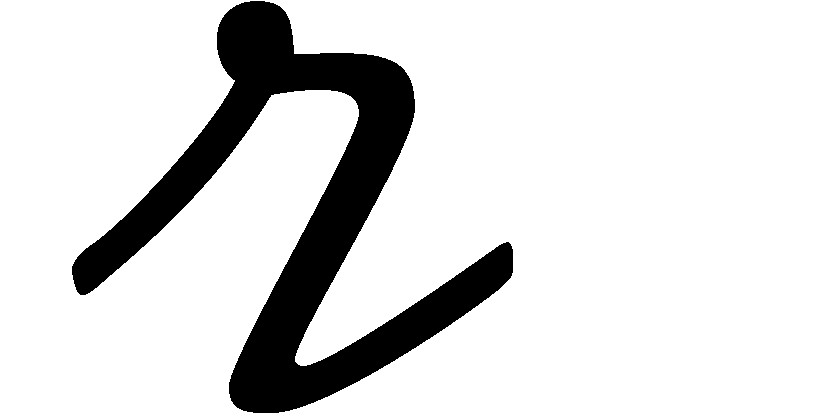
\includegraphics[trim= 1em 0 14em 0,clip]{fonts/ScriptR}}$}}= \vec{r} - \vec{w}(t_r)$%
\lthtmlindisplaymathZ
\lthtmlcheckvsize\clearpage}

{\newpage\clearpage
\lthtmlinlinemathA{tex2html_wrap_indisplay4345}%
$\displaystyle V(\vec{r}, t) = \frac{1}{4\pi\epsilon_0}    \frac{q}{\left| {\mbox{$\resizebox{.09in}{.08in}{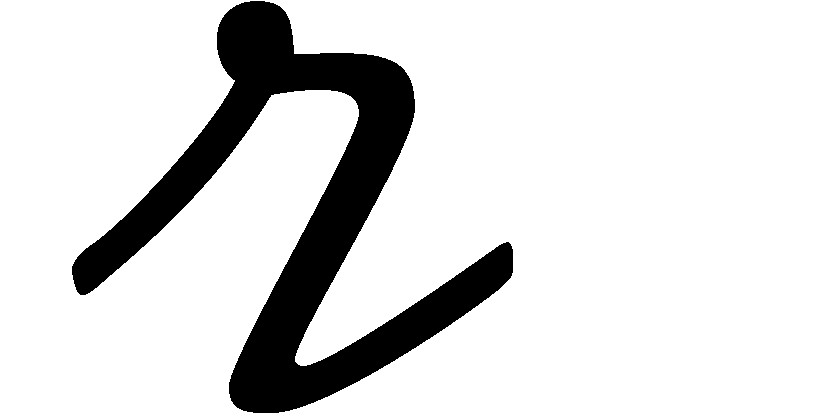
\includegraphics[trim= 1em 0 14em 0,clip]{fonts/ScriptR}}$}}- {\mbox{$\resizebox{.09in}{.08in}{
\includegraphics[trim= 1em 0 14em 0,clip]{fonts/BoldR}}$}}\cdot \vec{\beta} \right|}$%
\lthtmlindisplaymathZ
\lthtmlcheckvsize\clearpage}

{\newpage\clearpage
\lthtmlinlinemathA{tex2html_wrap_indisplay4348}%
$\displaystyle \vec{A}(\vec{r}, t) = \frac{1}{4\pi\epsilon_0}    \frac{q\vec{v}}{\left| {\mbox{$\resizebox{.09in}{.08in}{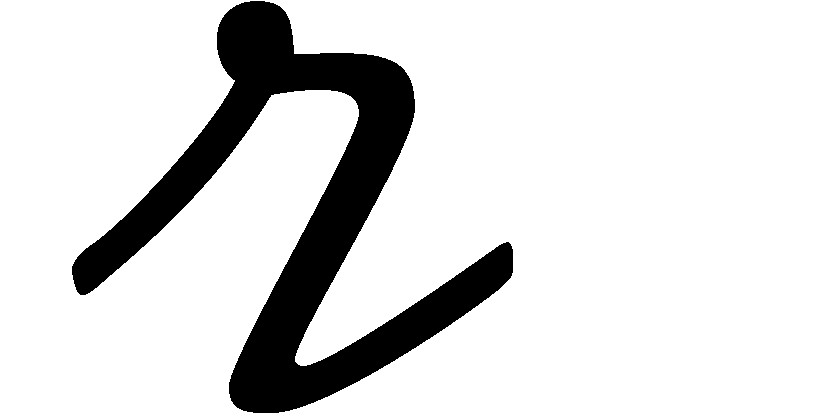
\includegraphics[trim= 1em 0 14em 0,clip]{fonts/ScriptR}}$}}- {\mbox{$\resizebox{.09in}{.08in}{
\includegraphics[trim= 1em 0 14em 0,clip]{fonts/BoldR}}$}}\cdot \vec{\beta} \right|} \;.$%
\lthtmlindisplaymathZ
\lthtmlcheckvsize\clearpage}

\stepcounter{section}
{\newpage\clearpage
\lthtmlinlinemathA{tex2html_wrap_inline4351}%
$ \vec{E}(t)=\vec{E}_0 e^{-i\omega t}$%
\lthtmlindisplaymathZ
\lthtmlcheckvsize\clearpage}

{\newpage\clearpage
\lthtmlinlinemathA{tex2html_wrap_inline4353}%
$ \vec{B}(t)=\vec{B}_0 e^{-i\omega t}=\frac{1}{c} \hat{\vec{k}}\times \vec{E}_0e^{-i\omega t}$%
\lthtmlindisplaymathZ
\lthtmlcheckvsize\clearpage}

{\newpage\clearpage
\lthtmlinlinemathA{tex2html_wrap_indisplay4354}%
$\displaystyle \left\langle \vec{S} \right\rangle  = \frac{1}{T}\int_0^{T}\frac{1}{\mu_0} \Re\{ \vec{E} \}\times \Re\{ \vec{B} \} dt \;,$%
\lthtmlindisplaymathZ
\lthtmlcheckvsize\clearpage}

{\newpage\clearpage
\lthtmlinlinemathA{tex2html_wrap_indisplay4355}%
$\displaystyle \Re\{\vec{E}\} = \frac{1}{2} (\vec{E} + \vec{E}^*)$%
\lthtmlindisplaymathZ
\lthtmlcheckvsize\clearpage}

{\newpage\clearpage
\lthtmlinlinemathA{tex2html_wrap_indisplay4356}%
$\displaystyle \left\langle \vec{S} \right\rangle  = \frac{1}{T}\int_0^{T} \frac{1}{\mu_0}\frac{1}{2} (\vec{E} + \vec{E}^*)\times \frac{1}{2} (\vec{B} + \vec{B}^*) dt \;.$%
\lthtmlindisplaymathZ
\lthtmlcheckvsize\clearpage}

{\newpage\clearpage
\lthtmlinlinemathA{tex2html_wrap_inline4358}%
$ \vec{E}\times\vec{B}$%
\lthtmlindisplaymathZ
\lthtmlcheckvsize\clearpage}

{\newpage\clearpage
\lthtmlinlinemathA{tex2html_wrap_inline4360}%
$ \vec{E}^*\times\vec{B}^*$%
\lthtmlindisplaymathZ
\lthtmlcheckvsize\clearpage}

{\newpage\clearpage
\lthtmlinlinemathA{tex2html_wrap_inline4362}%
$ e^{-2i\omega t}$%
\lthtmlindisplaymathZ
\lthtmlcheckvsize\clearpage}

{\newpage\clearpage
\lthtmlinlinemathA{tex2html_wrap_indisplay4363}%
$\displaystyle \left\langle \vec{S} \right\rangle  = \frac{1}{\mu_0} \frac{1}{4} (\vec{E}\times\vec{B}^* +  \vec{E}^*\times\vec{B}) = \frac{1}{2\mu_0}\Re\{ \vec{E}\times\vec{B}^*\}\;.$%
\lthtmlindisplaymathZ
\lthtmlcheckvsize\clearpage}

{\newpage\clearpage
\lthtmlinlinemathA{tex2html_wrap_inline4365}%
$ \vec{B}=\frac{1}{c}\hat{\vec{k}}\times \vec{E}$%
\lthtmlindisplaymathZ
\lthtmlcheckvsize\clearpage}

{\newpage\clearpage
\lthtmlinlinemathA{tex2html_wrap_indisplay4366}%
$\displaystyle \left\langle \vec{S} \right\rangle  = \frac{1}{2c\mu_0}\Re\{ \vec{E}\times(\hat{\vec{k}}\times\vec{E}^*)\} = \frac{1}{2c\mu_0} \left| E \right|^2 \hat{\vec{k}} = I\hat{\vec{k}} \;.$%
\lthtmlindisplaymathZ
\lthtmlcheckvsize\clearpage}

{\newpage\clearpage
\lthtmlinlinemathA{tex2html_wrap_inline4368}%
$ E$%
\lthtmlindisplaymathZ
\lthtmlcheckvsize\clearpage}

{\newpage\clearpage
\lthtmlinlinemathA{tex2html_wrap_inline4370}%
$ \vec{E}=\vec{E}_1 + \vec{E}_2$%
\lthtmlindisplaymathZ
\lthtmlcheckvsize\clearpage}

{\newpage\clearpage
\lthtmlinlinemathA{tex2html_wrap_inline4372}%
$ \vec{E}_1\cdot\vec{E}_2=0$%
\lthtmlindisplaymathZ
\lthtmlcheckvsize\clearpage}

{\newpage\clearpage
\lthtmlinlinemathA{tex2html_wrap_indisplay4375}%
$\displaystyle \left\langle \vec{S} \right\rangle  = \frac{1}{2c\mu_0}\Re\{ (\vec{E}_1 + \vec{E}_2)\times(\hat{\vec{k}}\times(\vec{E}_1 + \vec{E}_2)^*)\} \;.$%
\lthtmlindisplaymathZ
\lthtmlcheckvsize\clearpage}

{\newpage\clearpage
\lthtmlinlinemathA{tex2html_wrap_indisplay4376}%
$\displaystyle \vec{E}_1 \times(\hat{\vec{k}}\times \vec{E}_2^*) = 0 \;.$%
\lthtmlindisplaymathZ
\lthtmlcheckvsize\clearpage}

{\newpage\clearpage
\lthtmlinlinemathA{tex2html_wrap_indisplay4377}%
$\displaystyle \left\langle \vec{S} \right\rangle  = \frac{1}{2c\mu_0} ( \left| \vec{E}_1 \right|^2 + \left| \vec{E}_2 \right|^2)\hat{\vec{k}}\;.$%
\lthtmlindisplaymathZ
\lthtmlcheckvsize\clearpage}

\stepcounter{section}
{\newpage\clearpage
\lthtmlinlinemathA{tex2html_wrap_indisplay4379}%
$\displaystyle f(\vec{q})  = \int \rho(r) \exp(-i \vec{q}\cdot\vec{r}) \; d^3r \; .$%
\lthtmlindisplaymathZ
\lthtmlcheckvsize\clearpage}

{\newpage\clearpage
\lthtmlinlinemathA{tex2html_wrap_inline4381}%
$ \vec{q} = q \hat{\vec{z}}$%
\lthtmlindisplaymathZ
\lthtmlcheckvsize\clearpage}

{\newpage\clearpage
\lthtmlinlinemathA{tex2html_wrap_inline4383}%
$ \vec{q}\cdot\vec{r} =  q r \cos\theta$%
\lthtmlindisplaymathZ
\lthtmlcheckvsize\clearpage}

{\newpage\clearpage
\lthtmlinlinemathA{tex2html_wrap_inline4385}%
$ q$%
\lthtmlindisplaymathZ
\lthtmlcheckvsize\clearpage}

{\newpage\clearpage
\lthtmlinlinemathA{tex2html_wrap_inline4387}%
$ r$%
\lthtmlindisplaymathZ
\lthtmlcheckvsize\clearpage}

{\newpage\clearpage
\lthtmlinlinemathA{tex2html_wrap_indisplay4388}%
$\displaystyle f(\vec{q})$%
\lthtmlindisplaymathZ
\lthtmlcheckvsize\clearpage}

{\newpage\clearpage
\lthtmlinlinemathA{tex2html_wrap_indisplay4389}%
$\displaystyle = \int_0^{2\pi} d\phi \int_0^\infty \rho(r) r^2 dr \int_0^\pi
\sin\theta d\theta  \exp(-i q r \cos\theta)$%
\lthtmlindisplaymathZ
\lthtmlcheckvsize\clearpage}

{\newpage\clearpage
\lthtmlinlinemathA{tex2html_wrap_indisplay4390}%
$\displaystyle =2\pi \int_0^\infty \rho(r) r^2 dr \int_{-1}^1  d\cos\theta  \exp(-i q r
\cos\theta)$%
\lthtmlindisplaymathZ
\lthtmlcheckvsize\clearpage}

{\newpage\clearpage
\lthtmlinlinemathA{tex2html_wrap_indisplay4391}%
$\displaystyle =2\pi \int_0^\infty \rho(r) r^2 dr \frac{1}{-iqr}\int_{iqr}^{-iqr}  du  \exp(u)$%
\lthtmlindisplaymathZ
\lthtmlcheckvsize\clearpage}

{\newpage\clearpage
\lthtmlinlinemathA{tex2html_wrap_indisplay4392}%
$\displaystyle =2\pi \int_0^\infty \rho(r) r^2 dr \frac{\exp(iqr) - \exp(-iqr)}{iqr}$%
\lthtmlindisplaymathZ
\lthtmlcheckvsize\clearpage}

{\newpage\clearpage
\lthtmlinlinemathA{tex2html_wrap_indisplay4393}%
$\displaystyle f(q)$%
\lthtmlindisplaymathZ
\lthtmlcheckvsize\clearpage}

{\newpage\clearpage
\lthtmlinlinemathA{tex2html_wrap_indisplay4394}%
$\displaystyle = \int_0^\infty \rho(r)   \frac{\sin(qr)}{qr}  4\pi r^2 dr$%
\lthtmlindisplaymathZ
\lthtmlcheckvsize\clearpage}


\end{document}
